%!TEX TS-program = pdflatex
\documentclass[12pt]{article}
\usepackage[noblocks]{authblk}

\usepackage{lineno}
\renewcommand{\linenumberfont}{\normalfont\bfseries\small}
\linenumbers
\usepackage{amsmath, amssymb}
\usepackage[T1]{fontenc}
\usepackage[utf8]{inputenc}
\usepackage{mathptmx}
\usepackage{hyperref, fixltx2e, gensymb, natbib, wrapfig, graphicx, caption, subcaption, pifont}
\usepackage{longtable, array}
\usepackage{xcolor}
\newcommand{\red}[1]{\textcolor{red}{#1}}
\usepackage[a4paper, margin=2cm]{geometry}
% \fontsize{10.8pt}{2cm}\selectfont
\usepackage{soul}
\renewcommand{\baselinestretch}{2}

\usepackage[export]{adjustbox}

\usepackage[utf8]{inputenc}
\usepackage{fancyhdr}
\usepackage[shortlabels]{enumitem}

\setcounter{secnumdepth}{4}
\date{}
\usepackage[compact]{titlesec}
\titlespacing{\section}{0pt}{-1.0ex}{-1.0ex}
\titlespacing{\subsection}{0pt}{1ex}{0ex}
\titlespacing{\subsubsection}{0pt}{0.5ex}{0ex}

\bibliographystyle{mee}
\usepackage[font=small,labelfont=bf]{caption}
\graphicspath{ {../figures/original_v1_figures/} {../figures/new_physical_model_figures/} {../figures/new_dnn_and_ablation_figures/} }

\setlength{\parskip}{0.5em}

% This part is used to avoid hyphenation (can be helpful when need to convert to Word for submission)
\tolerance=1
\emergencystretch=\maxdimen
\hyphenpenalty=10000
\hbadness=10000

\begin{document}

\title{\normalsize\textbf {Spatially Aware Deep Learning for Microclimate Prediction from High-Resolution Geospatial Imagery}}

\author[1]{\normalsize Idan Sulami}
\author[1]{\normalsize Alon Itzkovitch}
\author[2]{\normalsize Michael R. Kearney}
\author[3]{\normalsize Moni Shahar}
\author[1,*]{\normalsize Ofir Levy}

\affil[1]{\normalsize Tel Aviv University, Faculty of Life Sciences, School of Zoology, Tel Aviv, Israel}
\affil[2]{\normalsize School of BioSciences, The University of Melbourne, Melbourne, Victoria, Australia}
\affil[3]{\normalsize Tel Aviv University, Center for Artificial Intelligence \& Data Science, Tel Aviv, Israel}

\maketitle 

\noindent \textbf{*Corresponding author:} Ofir Levy; mailing address: School of Zoology, Faculty of Life Sciences, Tel Aviv University, 6997801, Israel; phone: +972504384717; fax: +97236409403; email: levyofir@tauex.tau.ac.il.

\section*{ABSTRACT}
\noindent
Microclimate models link climate to the conditions organisms experience, yet most physically based frameworks compute ground temperature column by column, treating each spatial unit as thermally independent of its surroundings. How far surrounding terrain shapes local microclimates, and whether this independence assumption matters, remains unquantified in heterogeneous landscapes. We addressed both questions in a desert landscape by combining a convolutional neural network (CNN) with a process-based physical model. Using drone-derived maps of obstacle height, vegetation greenness, shade, skyview factor, and incoming solar radiation at 15~cm resolution, we trained the CNN to predict ground surface temperature at a focal pixel while varying the square input tile width from a single pixel (0.15~m) to 12.2~m at a fixed parameter count. Surrounding terrain reduced midday mean squared error (MSE) by about 38\% in both open sand and canopy shade, with gains leveling off at tile widths of 1.7--2.8~m (0.9--1.4~m from the target pixel) and stabilizing by 4.7~m, a scale comparable to desert shrubs and their shadows. Larger tiles did not significantly improve morning or evening predictions, when the ground surface is nearly isothermal under low sun. At midday, feature permutations showed that the predictive gain from surrounding terrain came primarily from incoming solar radiation, followed by skyview factor, shade, and obstacle height. We then tested whether horizontal heat transport could explain this spatial dependence. Whereas drone thermal measurements showed shaded bare ground only 1--3$^\circ$C cooler than sunlit sand at midday, a one-dimensional (1D) energy-balance model predicted differences of 5--12$^\circ$C. Adding near-surface horizontal heat advection and a neutral-stability turbulent mixing floor reduced shaded-ground MSE by 70.2\% across evaluation flights (lowering error in 31 of 32 shaded submaps) while leaving open-ground predictions nearly unchanged. The physical model's advective relaxation distance (0.4--1.4~m) and the CNN's plateau half-width (0.9--1.4~m) both point to spatial interactions at the 1--3~m scale of individual shrubs. These findings indicate that the spatial-independence assumption breaks down across small shade boundaries, that omitting lateral heat exchange accounts for much of the shade-cooling bias in 1D models, and that fixed-capacity neural networks can help identify the spatial scales over which microclimatic processes act.

\noindent \textbf{Keywords:} landscape, modeling, drone, climate, neural networks, management, rocks, vegetation.

\section{INTRODUCTION}

\noindent Climate shapes how organisms experience their environment across scales, from momentary behavioral decisions of individuals to long-term community and evolutionary processes \citep{potter_2013, pincebourde_2020}. However, studying these impacts is challenging because organisms experience conditions within centimeters to meters of their bodies, whereas standard meteorological observations and gridded climate datasets are much coarser ($>10$~km) \citep{kearney_2012}. For terrestrial ectotherms and small ground-dwelling animals, body temperatures and activity periods depend strongly on the bare ground surface skin temperature ($T_g$) of local microhabitats \citep{bakken_1992, huey_1976}. In arid environments, intense solar heating drives exposed ground temperatures above preferred thermal ranges, forcing animals to shuttle into shaded refuges beside rocks, boulders, and sparse shrubs \citep{sears_2011, Stark_2023}. Predicting ground temperatures within these shaded refuges is therefore essential for assessing thermal stress and habitat suitability as the climate warms.

To bridge the gap between coarse climate data and organismal experience, ecologists use mechanistic microclimate models that solve the surface energy balance between the ground, the soil, and the atmosphere \citep{campbell_1998, kearney_2017, maclean_2019}. Although current frameworks account for topographic shading and sky exposure using detailed terrain maps \citep{kearney_2020}% , maclean_2026
, they still compute turbulent heat fluxes column by column (1D), calculating each location's vertical energy balance as if the near-surface air were horizontally uniform. This independence assumption is questionable across small shaded patches, where steep temperature gradients ($>10^\circ\text{C}$ over meters) between sunlit and shaded ground drive horizontal heat exchange. Wind blowing across hot open terrain advects warm air into adjacent shade \citep{oke_1987, campbell_1998}, while turbulent eddies generated over the surrounding sunlit landscape maintain vertical mixing across narrow shadows \citep{helgason_2012}. By omitting horizontal heat transport, 1D column models can overestimate the cooling provided by isolated shade \citep{Itzkovitch2025}. Although drone-based remote sensing now maps topography, vegetation, and surface temperatures at centimeter resolution \citep{duffy_2021}, the distance over which surrounding terrain influences local ground temperature, and the extent to which adding lateral advection improves physical predictions, remain poorly quantified.

Quantifying this spatial scale directly from field observations requires a method that captures nonlinear spatial interactions without prescribing their functional form in advance. Convolutional neural networks (CNNs) are well-suited for this task \citep{lecun_2015, campsvalls_2025}, particularly when high-resolution drone maps are paired with local meteorological measurements \citep{slater_2023, levy_2024}. Here, we used a CNN to test how the size of the surrounding input area affects ground temperature predictions across open and shaded microhabitats, times of day, and environmental map layers. We varied the square input tile width from a single pixel to $81\times81$ pixels ($0.15$ to $12.15$~m) while keeping the network architecture and parameter count fixed, ensuring that accuracy gains reflected added spatial information rather than increased model capacity. To test a physical mechanism for the observed spatial dependence, we then compared a 1D surface energy-balance model \citep{Itzkovitch2025} against a 2D version that adds near-surface horizontal heat advection and turbulent mixing across shadow margins.% and \textit{microclimf} \citep{maclean_2026}.

We hypothesized that: (1) surrounding terrain information improves ground surface temperature predictions, particularly in shaded microhabitats, up to a characteristic distance beyond which gains level off; and (2) accounting for lateral heat exchange in a process-based energy-balance model substantially reduces the overestimation of shade cooling in the 1D baseline model.

\section{MATERIALS AND METHODS}
\subsection{General Approach}
\noindent 
To quantify how surrounding terrain shapes local ground temperatures, we combined a convolutional neural network (CNN) with a physical energy-balance model (Fig.~\ref{fig:complete_data_flow}). In the CNN, we systematically expanded the input tile width from a single pixel ($0.15$~m) to $12.15$~m while holding the parameter count constant, isolating how surrounding terrain improves ground surface temperature ($T_g$) predictions across microhabitats, times of day, and map layers. These predictions were evaluated on spatial blocks and flights excluded from training so that accuracy gains reflected generalizable spatial relationships rather than memorized sites. To test whether the spatial dependence identified by the CNN could be explained by horizontal heat transport, we then compared our physical energy-balance model with and without lateral heat advection and turbulent mixing across shade boundaries \citep{Itzkovitch2025}.% and the independent state-of-the-art package \textit{microclimf} \citep{maclean_2026}.

\begin{figure}
    \centering
    \begin{minipage}{0.6\textwidth}
        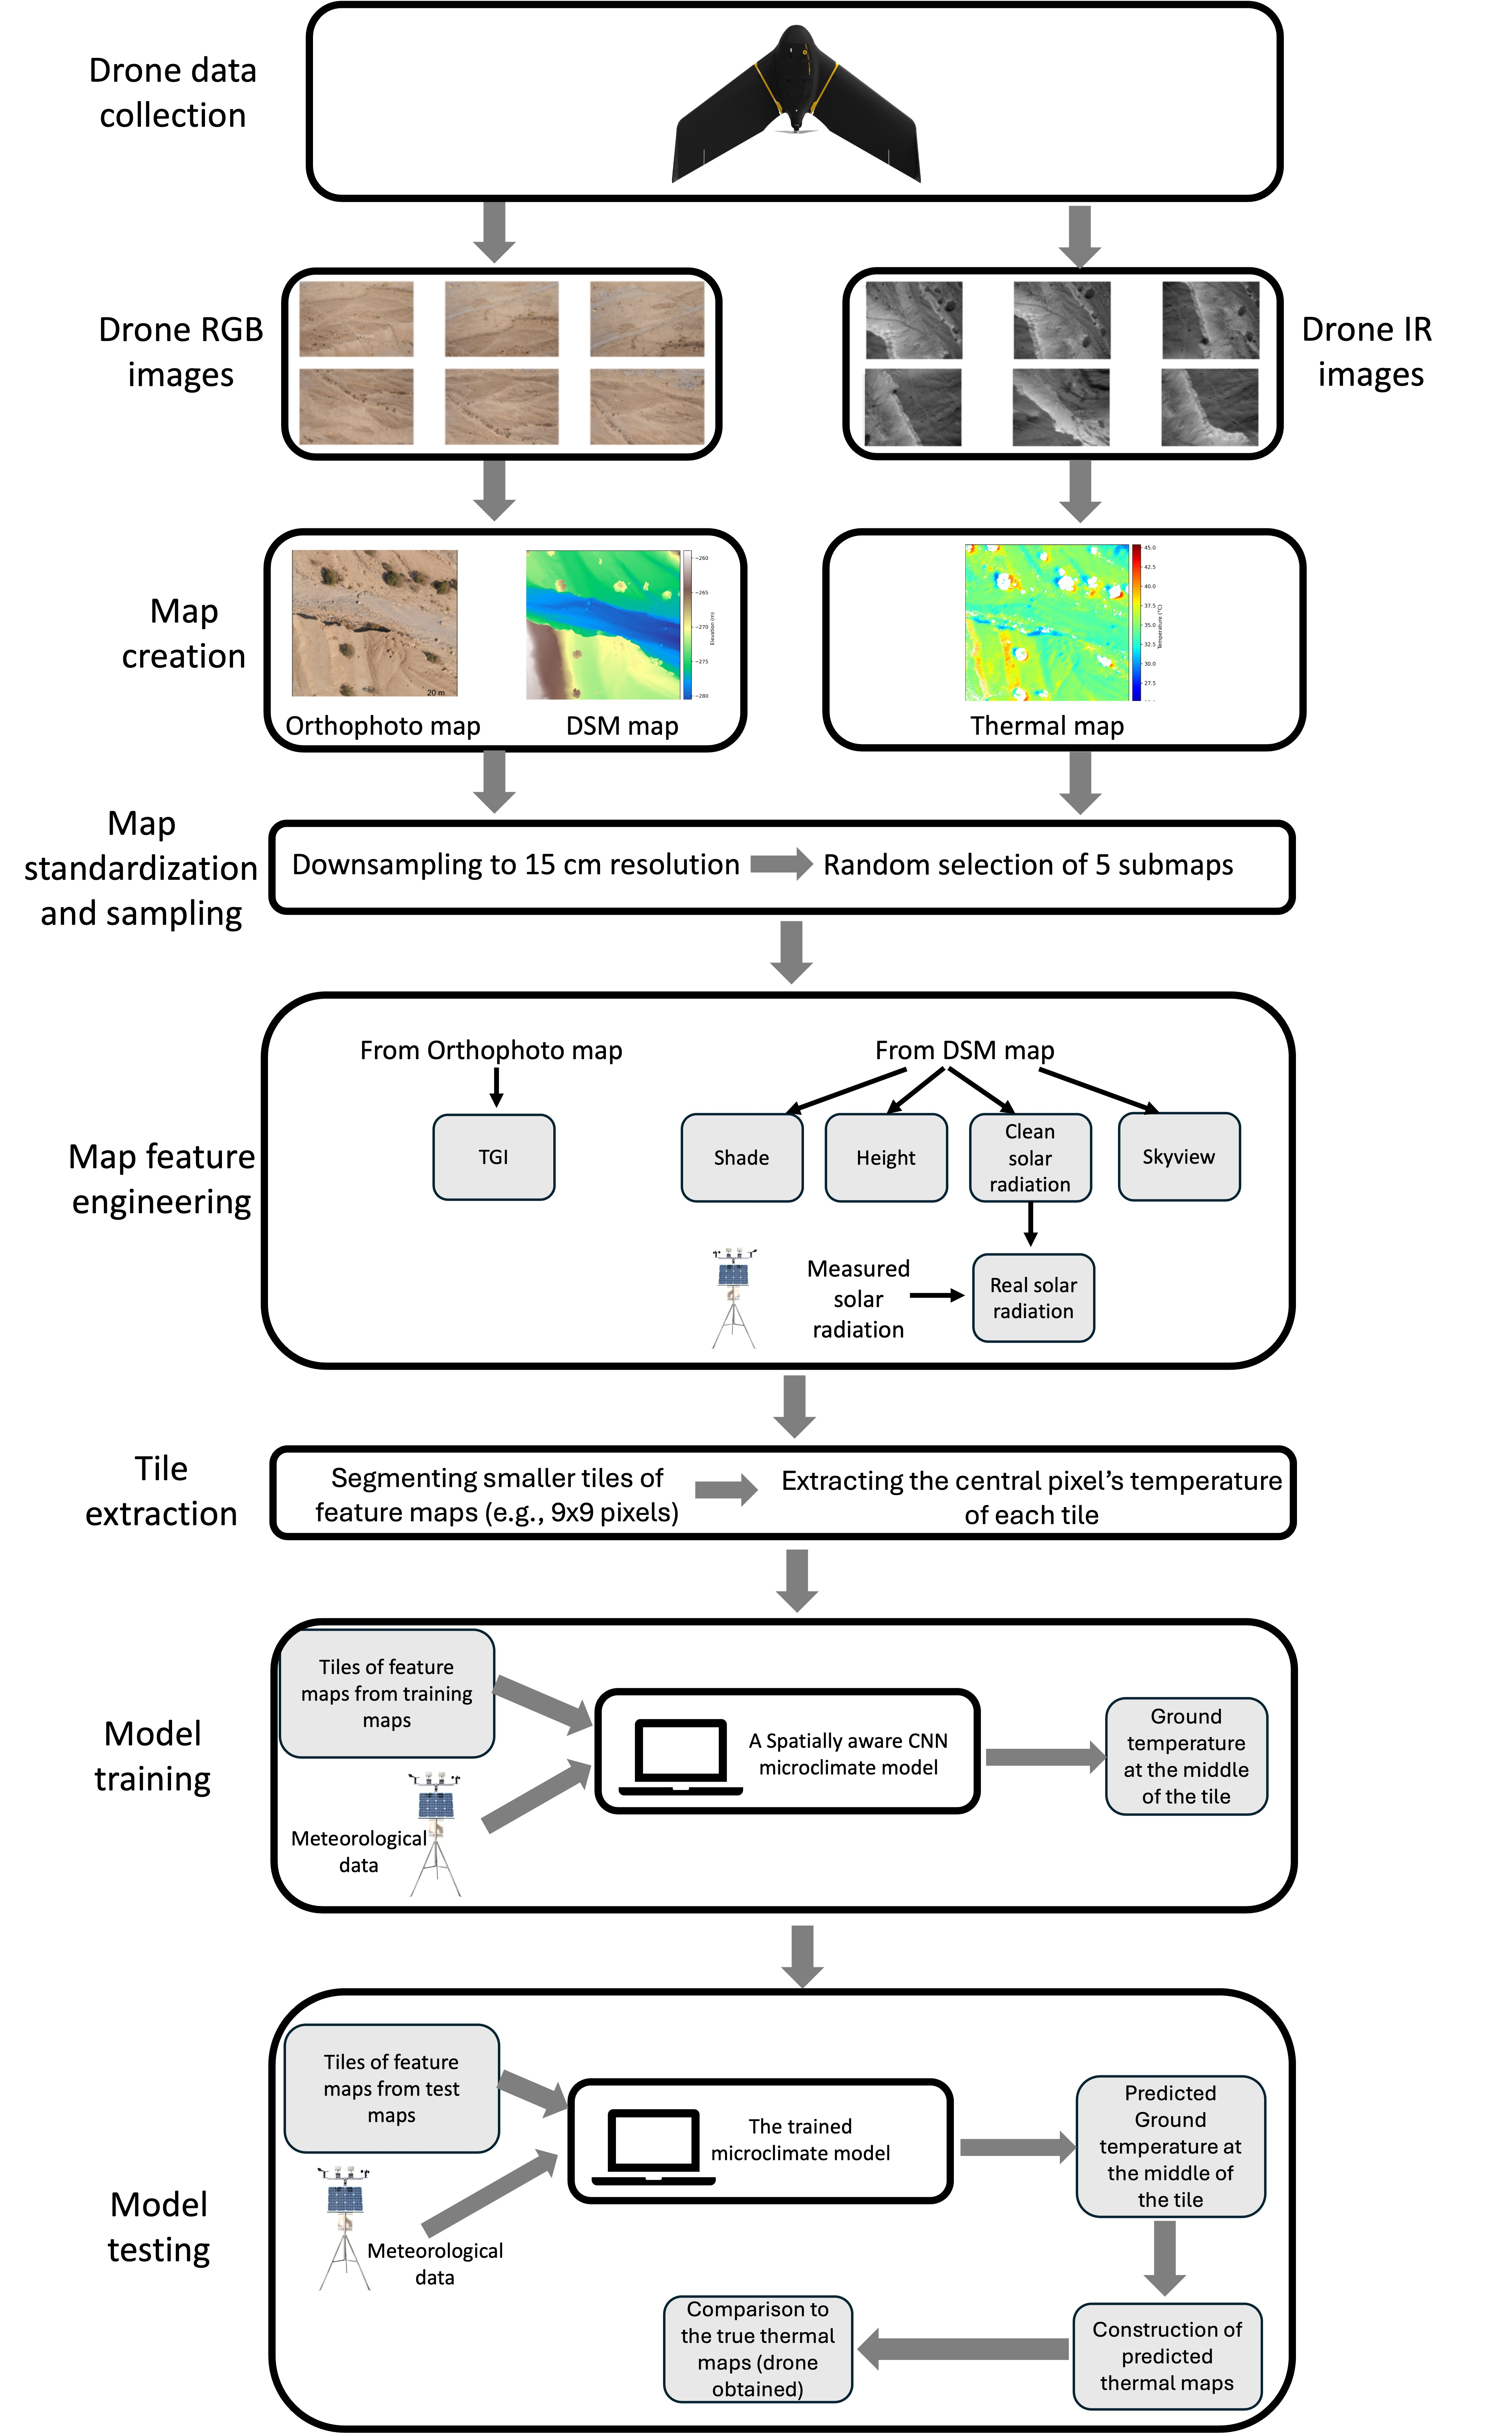
\includegraphics[width=\textwidth]{Sulami_Fig_1.jpg}
    \end{minipage}%
    \hfill
    \begin{minipage}{0.35\textwidth}
        \caption{Flowchart of the data and modeling pipeline. Drone surveys simultaneously collected RGB and thermal imagery, which were processed into orthophotos, Digital Surface Models (DSMs), and calibrated thermal maps at 15~cm resolution. Submaps were partitioned using a $50\times50$~m spatial blocking design. Five environmental predictor layers (Triangular Greenness Index [TGI], shade, obstacle height, skyview factor, and incoming solar radiation) were segmented into square tiles of increasing width ($0.15$ to $12.15$~m), paired with concurrent weather-station readings, and used to train a fixed-capacity CNN to predict ground temperature at the center pixel. Predictions were evaluated across microhabitats, times of day, and feature ablations, and compared with physical energy-balance models with and without lateral heat exchange.
        }
        \label{fig:complete_data_flow}
    \end{minipage}
\end{figure}

\subsection{Study Site and Field Data Collection}

\paragraph*{\textit{Study Site}} We collected field data in the Judean Desert, Israel (31°21'N, 35°21'E), adjacent to the Dead Sea basin (~240--400~m below sea level). This hyper-arid landscape consists of alluvial plains, rocky slopes, and wadi beds with sparse perennial shrubs and seasonal annuals \citep{moncaz_2012}. Within this region, our surveys focused on the Tse'elim River alluvial fan (31°21'04.8"N, 35°21'11"E), which is covered by gravelly sand, scattered limestone rocks, and sparse shrub cover ($\approx 5\%$). In summer, exposed bare ground temperatures rise from approximately 30°C in early morning to $>45$°C at midday, whereas shaded ground beneath rocks and shrubs remains cooler (~37°C) \citep{levy_2016a}. In winter, midday temperatures reach ~27°C on open ground and ~25°C in shade.

\paragraph*{\textit{Target Microclimate Definition and Thermal Calibration}}
We defined our modeling target as bare ground surface skin temperature ($T_g$, $^\circ$C), which integrates the radiative, convective, conductive, and evaporative heat exchanges experienced by ground-dwelling organisms \citep{bakken_1992}. To map $T_g$ across the site, we collected radiometric thermal imagery (15~cm resolution) alongside RGB imagery using an eBee~X fixed-wing drone equipped with a Duet~T dual camera (SenseFly, Switzerland). Because uncooled thermal sensors (nominal factory accuracy $\pm 5^\circ$C) are subject to camera drift and atmospheric attenuation, each thermal map was offset-corrected to match concurrent ground surface temperatures recorded by contact and infrared sensors over exposed bare sand at our mobile weather station. To restrict evaluation to bare ground, we excluded pixels with active vegetation cover (Triangular Greenness Index, $\text{TGI} > 0.04$).

\paragraph*{\textit{Meteorological Data Collection}}
During every flight, a portable weather station (MaxiMet GMX501, GILL Instruments, UK) positioned in a flat, unshaded sand patch recorded solar irradiance, air temperature, relative humidity, atmospheric pressure, wind speed, wind direction, and surface and canopy temperatures at 10-minute intervals. These on-site readings were supplemented with regional albedo and soil moisture and temperature profiles from the Global Land Data Assimilation System (GLDAS; \citealt{TheGlobalLandDataAssimilationSystem}) and hourly atmospheric forcing from ERA5-Land reanalysis for the physical model (Table~\ref{table:physparam}). In total, we conducted 33 drone flights across eight field campaigns between May 2019 and May 2021, spanning morning to evening conditions (Supplementary Table~S1).

\subsection{Spatial Predictor Maps and Dataset Preparation}

\noindent We processed the drone RGB imagery in Pix4DMapper (v4.23, Pix4D Inc., USA) to generate 3~cm orthophotos, Digital Surface Models (DSMs), and Digital Terrain Models (DTMs), and resampled all layers to the 15~cm ($0.15$~m) grid of the calibrated thermal maps. From these products, we derived five spatial predictor layers for each submap (detailed in Supplementary Section~S1):
\begin{enumerate}[leftmargin=*, nosep]
    \item \textbf{Incoming Solar Radiation (W~m$^{-2}$):} Total shortwave irradiance (direct beam and diffuse skylight) computed from the DSM using the \textit{r.sun} module in GRASS GIS \citep{GRASS_GIS_software, BIVAND20001043} (accounting for local slope, aspect, and horizon shading) and scaled to the weather-station pyranometer to adjust for cloud cover;
    \item \textbf{Shade (0 or 1):} Binary indicator of whether each pixel was shaded from the direct solar beam (1) or sunlit (0) at the time of the flight;
    \item \textbf{Skyview Factor (0--1):} The fraction of the sky hemisphere visible from each pixel, computed from the DSM using \textit{r.skyview} to quantify obstruction of diffuse skylight and longwave radiation by surrounding relief;
    \item \textbf{Obstacle Height (m):} Height of surface features above the surrounding bare ground ($\text{DSM} - \text{DTM}$), capturing rocks and shrubs;
    \item \textbf{Vegetation Index (TGI):} Triangular Greenness Index derived from RGB reflectance \citep{star_2020}, used as an indicator of green vegetation cover.
\end{enumerate}

\begingroup\small\renewcommand{\baselinestretch}{1.0}\selectfont
\renewcommand{\arraystretch}{1.15}
\setlength{\tabcolsep}{3pt}
\begin{longtable}{@{}>{\raggedright\arraybackslash}p{3.2cm}>{\raggedright\arraybackslash}p{1.8cm}>{\raggedright\arraybackslash}p{1.2cm}>{\raggedright\arraybackslash}p{4.4cm}>{\raggedright\arraybackslash}p{3.8cm}@{}}
\caption{Input variables of the deep learning model (DNN) and the physical energy-balance model. The five map layers are shared by both models. The eight weather inputs of the DNN overlap partly with those of the physical model, which additionally requires regional albedo, initial soil temperatures, prescribed soil moisture profiles, and atmospheric forcing parameters. All DNN inputs are standardised before training (Supplementary Section~S2.1).}
\label{table:physparam}\\
\hline
Variable & Units & DNN & Physical model & Source \\
\hline
\endfirsthead
\hline
Variable & Units & DNN & Physical model & Source \\
\hline
\endhead
\hline
\endfoot
\multicolumn{5}{@{}l}{\textbf{A. Map layers at 15~cm resolution (shared by both models)}} \\
\hline
Height ($H$) & m & Yes & Yes, per pixel & DSM $-$ DTM (Section~S1.5) \\
Shade presence (\textit{SHD}) & 0 or 1 & Yes & Yes, per pixel & GRASS \textit{r.sun} (Section~S1.2) \\
Solar radiation ($S$) & W\,m$^{-2}$ & Yes & Yes, per pixel & GRASS \textit{r.sun} (Section~S1.1) \\
Skyview factor (\textit{SVF}) & 0--1 & Yes & Yes, per pixel & GRASS \textit{r.skyview} (Section~S1.3) \\
Vegetation cover (\textit{TGI}) & index & Yes & Yes, per pixel & RGB orthophoto (Section~S1.4) \\
\hline
\multicolumn{5}{@{}l}{\textbf{B. Weather-station readings at flight time}} \\
\hline
Wind speed & m\,s$^{-1}$ & Yes & Yes, reduced by canopy drag and shade & Weather station (Section~2.1) \\
Wind direction & degrees & Yes, measured & Yes, measured: 10-min vector average at flight time (advected air layer only) & Weather station \\
Air temperature & $\degree$C & Yes & Yes & Weather station \\
Relative humidity & \% & Yes & Indirectly, via specific humidity and air density & Weather station \\
Dew point & $\degree$C & Yes & No & Weather station \\
Air pressure & hPa & Yes & Yes & Weather station \\
Solar radiation (scalar) & W\,m$^{-2}$ & Yes & No (pixel-level layer used) & Weather station \\
Ground temperature at station & $\degree$C & Yes & Starting value of iteration only & Weather station \\
Canopy-air and veg.~temp. & $\degree$C & No & Yes & Weather station \\
\hline
\multicolumn{5}{@{}l}{\textbf{C. Additional inputs of the physical model only}} \\
\hline
Albedo ($\alpha$) & \% & No & Yes, one value per flight & GLDAS (Section~2.1) \\
Soil temp.~at 10, 40, 100, 200~cm & K & No & Yes, initialises soil profile & GLDAS (Section~2.1) \\
Soil moisture at 10, 40, 100, 200~cm & m$^3$\,m$^{-3}$ & No & Yes, prescribed (top 3~cm set to 1/3 of 10~cm value) & GLDAS (Section~2.1) \\
Specific humidity and air density & kg\,kg$^{-1}$, kg\,m$^{-3}$ & No & Yes & Derived from air temp., humidity, pressure \\
Sky emissivity and cloud fraction & 0--1 & No & Yes, for downward longwave radiation & Pyranometer ratio; $\epsilon_{\text{sky}}$ from \citet{campbell_1998} \\
Hourly forcing (24~h before flight) & various & No & Yes, spin-up of soil profile & ERA5-Land adjusted to station \\
\hline
\multicolumn{5}{@{}l}{\textbf{D. Fixed parameters of the physical model}} \\
\hline
Ground and canopy emissivity & 0--1 & No & 0.95 & Constant \\
Soil texture & class & No & Noah-MP class 4 (silt loam): porosity 0.476, wilting 0.084 & Standard Noah-MP table \\
Roughness length and lateral parameters & & No & Listed in Supplementary Table~S4 & \\
\hline
\end{longtable}
\endgroup

\paragraph*{\textit{Spatial Blocking and Data Partitioning}}
To limit spatial autocorrelation between training and evaluation sets \citep{hastie2009elements, kuhn2013applied}, we divided the study area into non-overlapping $50\times50$~m blocks. Blocks were assigned to training (55\% of the area), validation (15\%), or hold-out test (30\%) sets based solely on non-thermal terrain covariates (slope, aspect, obstacle height, surface roughness, skyview factor, and TGI), so that all three sets sampled comparable terrain without using temperature data. Within each block, target pixel centers were kept at least $0.5$~m plus the half-width of the largest tile ($6.08$~m) inside the block boundary, preventing any input tile from crossing into a block with a different role. Alongside this spatial split, we partitioned the 33 flights temporally into 23 training/validation flights and 10 held-out test flights. Models were trained on the training blocks of the 23 training flights, monitored for early stopping on their validation blocks, and evaluated on the held-out test blocks of the 10 held-out flights.

\paragraph*{\textit{Sliding-Window Spatial Tiles}}
To test how the width of the surrounding input area affects temperature predictions, we extracted square tiles centered on each target pixel across eight neighborhood widths: $5\times5$ (0.75~m tile width), $9\times9$ (1.35~m), $15\times15$ (2.25~m), $21\times21$ (3.15~m), $31\times31$ (4.65~m), $47\times47$ (7.05~m), $63\times63$ (9.45~m), and $81\times81$ (12.15~m) pixels (Fig.~\ref{fig:tiles}), together with a single-pixel baseline ($1\times1$ pixel, 0.15~m). A square tile of width $W$ extends $W/2$ outward from the target pixel in each cardinal direction. Tiles were sampled by sliding a square window across the five stacked predictor maps in 5-pixel (0.75~m) steps horizontally and vertically, paired with concurrent weather-station readings, and standardized channel-wise using training-set means and standard deviations. Target ground temperatures were expressed as differences ($\Delta T_g$) from the mean temperature of flat, unshaded open ground ($<0.20$~m obstacle height) within the same submap to predict local temperature contrasts relative to open sand; this reference value can be added back to recover absolute temperatures (Supplementary Section~S2.1).

\begin{figure}
    \centering
    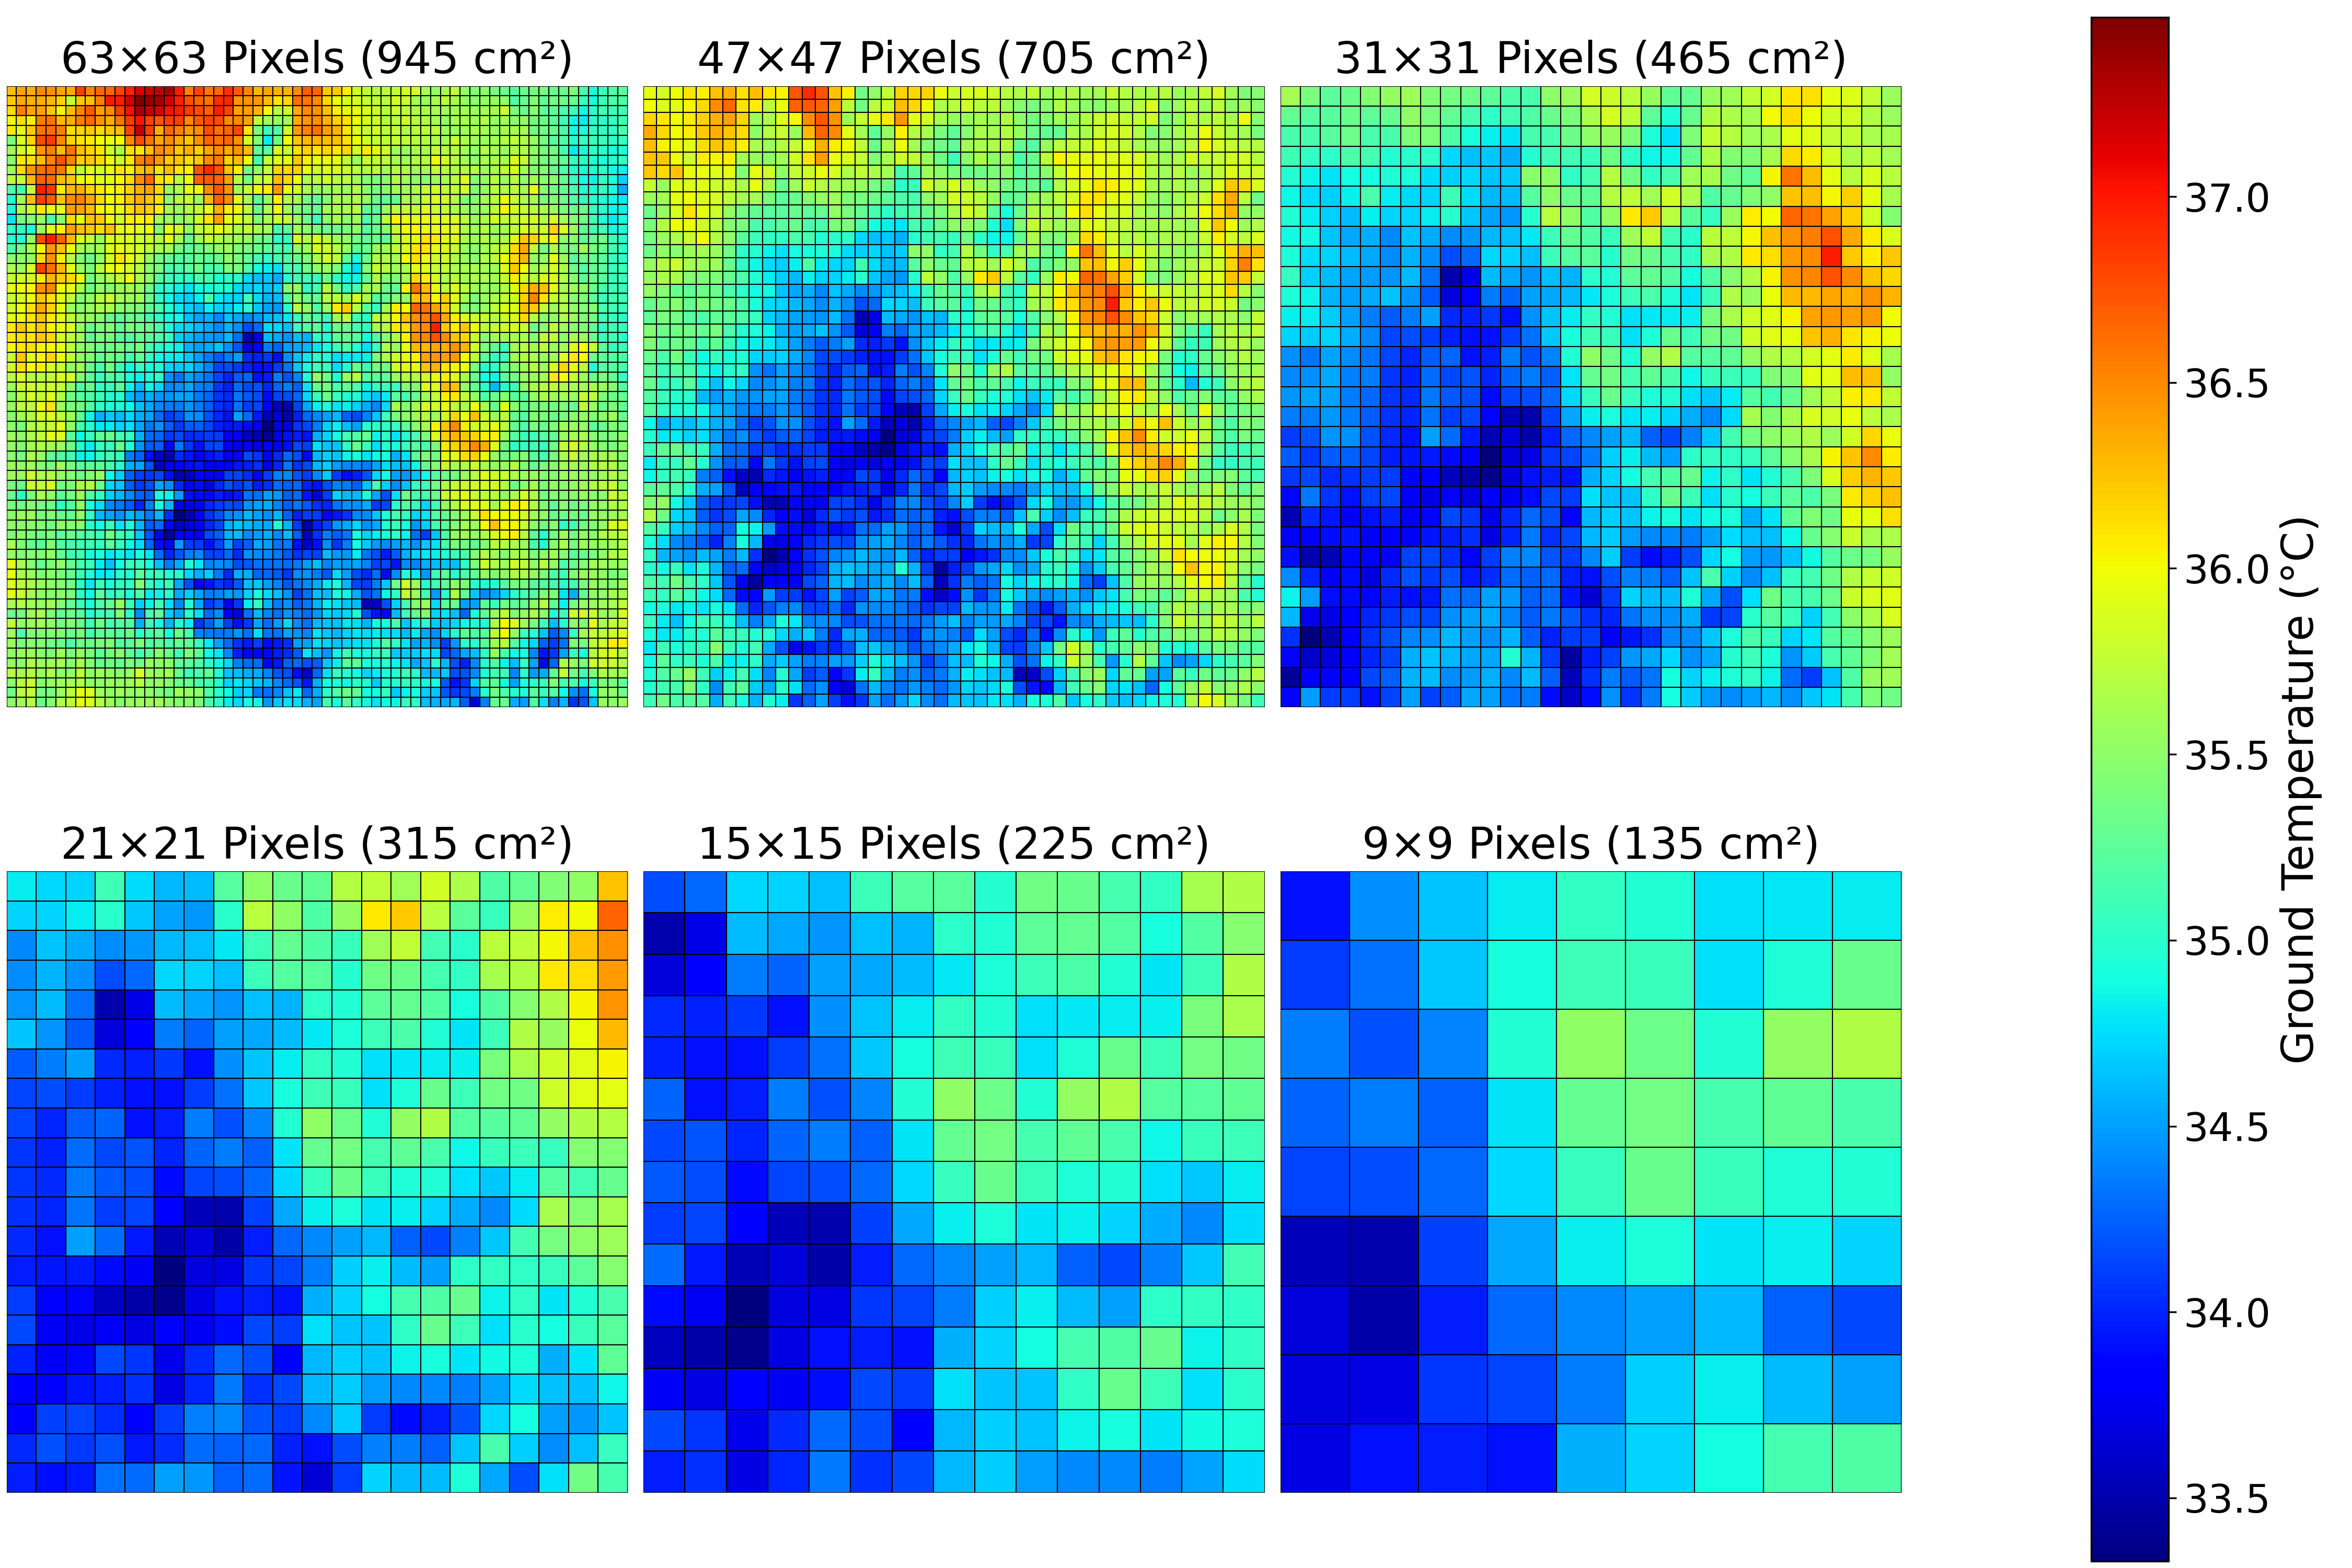
\includegraphics[width=1\textwidth]{Figure 2.png}
    \caption{Square input tiles of increasing width centered on a focal prediction pixel, ranging from $9\times9$ (1.35~m tile width) to $63\times63$ (9.45~m) pixels ($5\times5$ and $81\times81$ tiles omitted for clarity). Larger tiles provide broader surrounding terrain context, whereas smaller tiles restrict the model to local surface properties.}
    \label{fig:tiles}
\end{figure}

\subsection{Capacity-Controlled Convolutional Neural Network}

\noindent In standard convolutional networks, enlarging the input tile often increases the number of trainable parameters in downstream layers, confounding spatial extent with model capacity. We therefore designed a convolutional neural network (\texttt{FullResDilatedCNN}; Fig.~\ref{fig:architecture}; Supplementary Section~S2) that keeps the architecture and parameter count (55,729 parameters) identical across all nine tile widths.

\begin{figure}
    \centering
    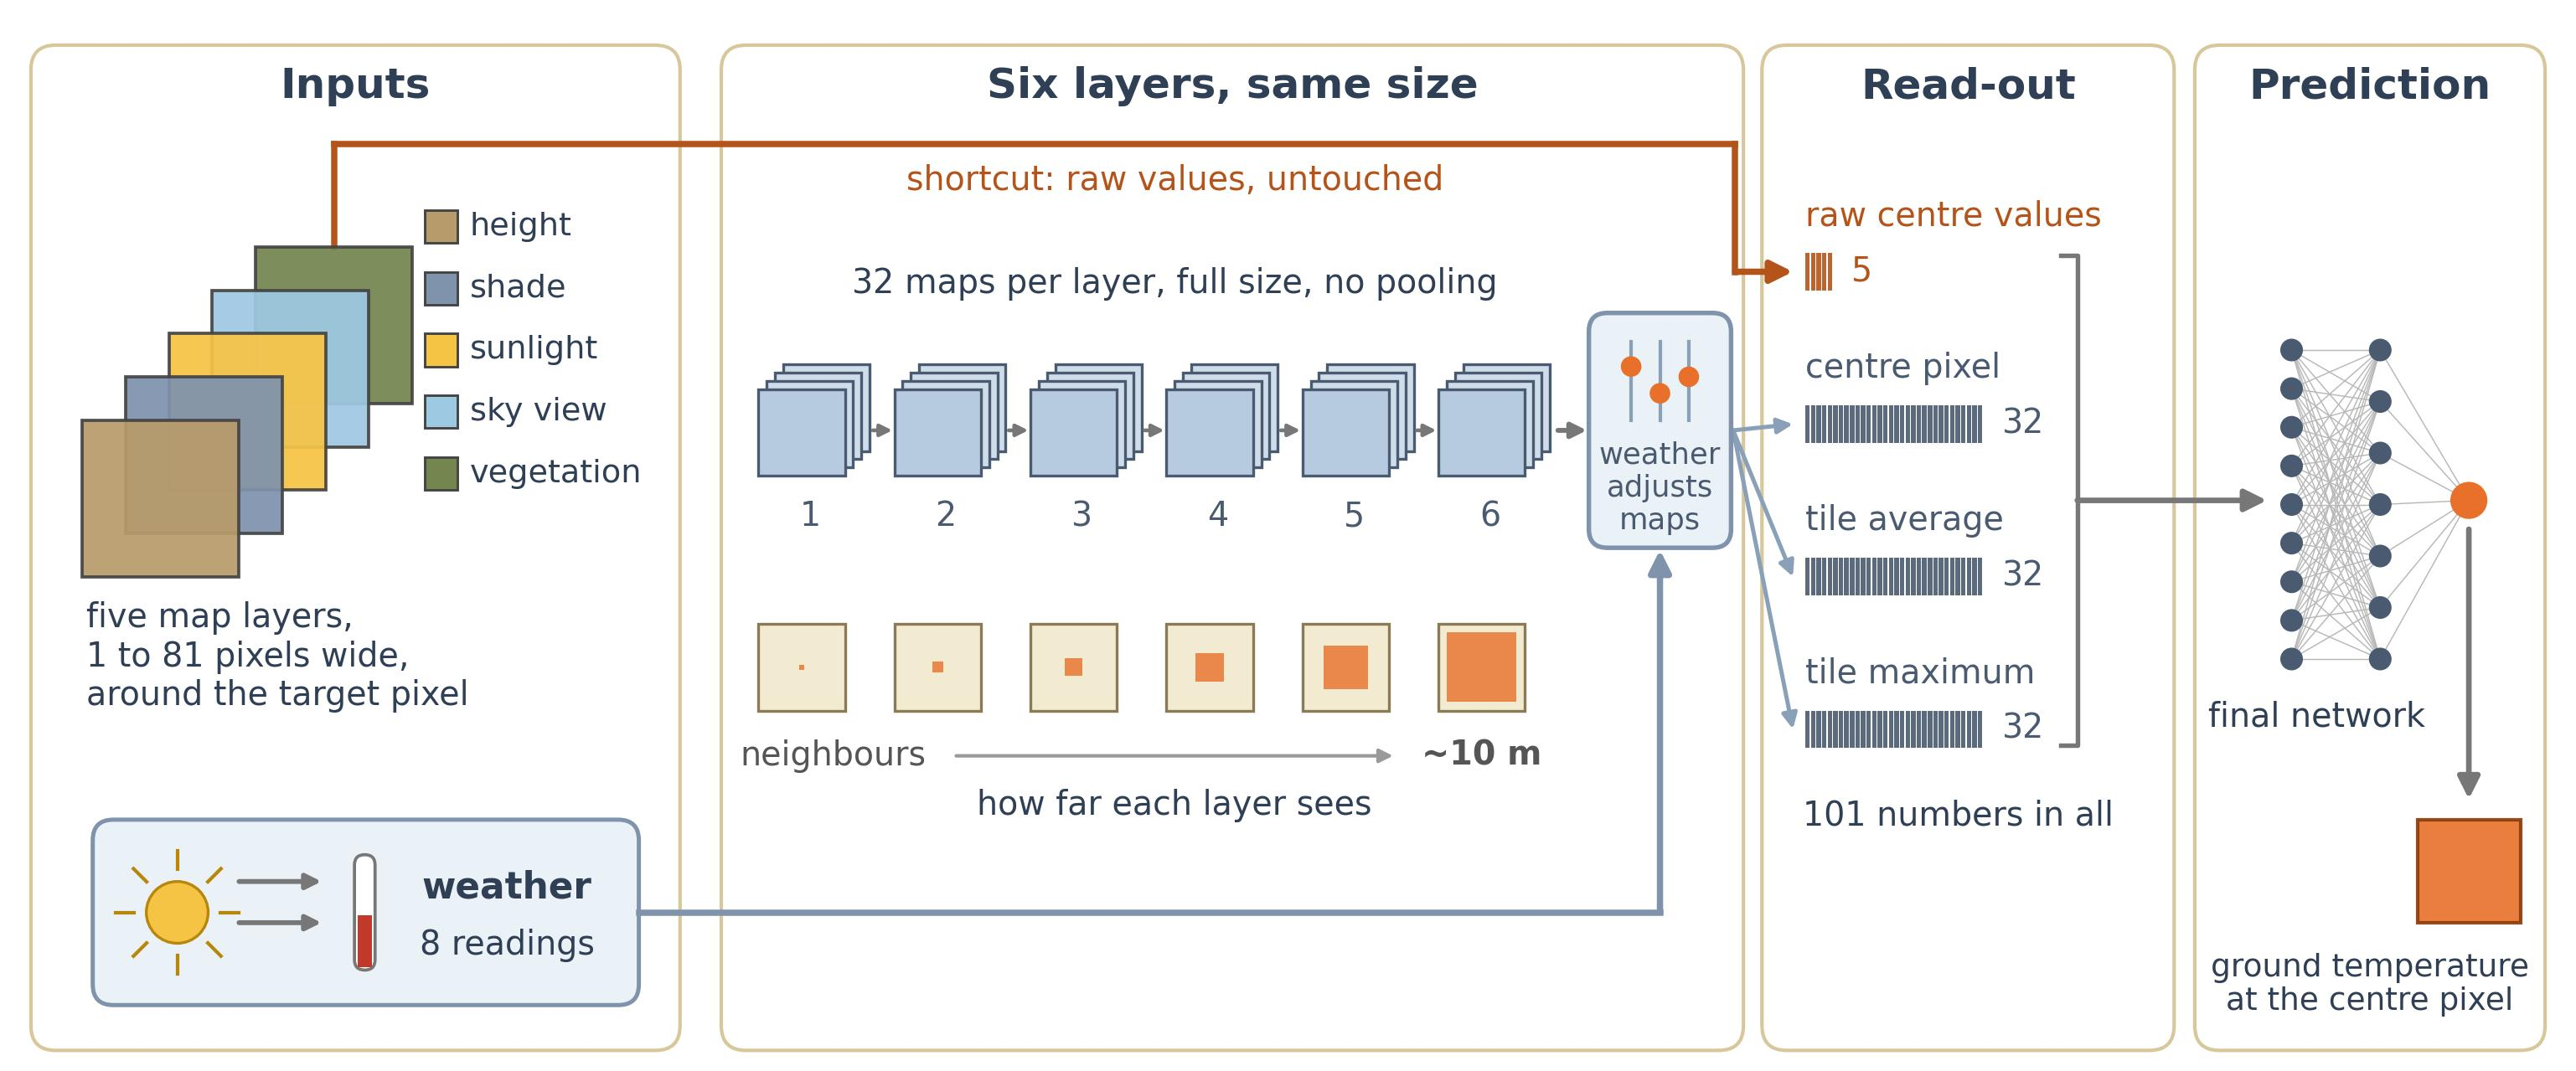
\includegraphics[width=1\textwidth]{Figure 3.jpg}
    \caption{Architecture of the capacity-controlled convolutional neural network. A five-layer input tile centered on the target pixel passes through six dilated convolutional layers in sequence. Each layer applies 32 filters and outputs 32 feature maps at the native 15~cm resolution (without spatial coarsening), spanning a receptive-field width of up to 65 pixels ($\approx 9.8$~m, or $\approx 4.8$~m outward from the center pixel). Eight flight-time weather readings modulate the 32 feature maps through learned per-channel scaling and shift factors (FiLM). The prediction head then concatenates the 32 modulated features at the center pixel, their tile-wide mean and maximum (32 values each), and a direct shortcut copy of the five raw map inputs at the center pixel (101 values in total) to predict the center pixel's temperature difference from open ground. Every tile width uses the same 55,729 parameters.
}
    \label{fig:architecture}
\end{figure}

\paragraph*{\textit{Network Architecture}}
Each five-layer input tile passes through six sequential $3\times3$ convolutional layers (32 channels each) with dilation factors of $1, 1, 2, 4, 8,$ and $16$ pixels. Dilating the filters expands the receptive field to a width of 65 pixels ($\approx 9.8$~m, extending $\approx 4.8$~m from the center pixel) without downsampling the 15~cm grid, preserving sharp shadow boundaries (Fig.~\ref{fig:architecture}). When a dilated filter reaches beyond the boundary of a smaller tile, outside positions are padded with zeros, which correspond to the training-set mean of each standardized feature. This zero-padding allows the same 55,729-parameter network to process any tile width from $1\times1$ to $81\times81$ without leaking information from outside the tile. Once the six convolutional layers extract the 32 spatial feature maps, an auxiliary two-layer network uses the eight flight-time weather variables (Table~\ref{table:physparam}B) to scale and shift each channel via Feature-wise Linear Modulation (FiLM). A final two-layer fully connected network then combines the 32 modulated features at the center pixel, their tile-wide mean and maximum (spatial pooling, 64 values), and a direct copy of the five raw center-pixel map values to predict the center pixel's temperature difference relative to open ground ($\Delta T_g$). Equations for every layer are provided in Supplementary Section~S2.2.

\paragraph*{\textit{Model Training}}
We trained the models using the AdamW optimizer (initial learning rate $\eta = 3 \times 10^{-5}$ with cosine annealing, weight decay $10^{-2}$, batch size 1024) for up to 200 epochs, minimizing a balanced absolute-error loss that weights open and shaded ground equally:
\begin{equation} 
\mathcal{L} = \frac{1}{2}\left(\frac{1}{N_\text{open}}\sum_{i \in \text{open}} \left|\Delta T_{i}^\text{obs} - \Delta T_{i}^\text{pred}\right| + \frac{1}{N_\text{shade}}\sum_{i \in \text{shade}} \left|\Delta T_{i}^\text{obs} - \Delta T_{i}^\text{pred}\right|\right),
\end{equation}
where $\Delta T_i^\text{obs}$ and $\Delta T_i^\text{pred}$ are the observed and predicted temperature differences from the submap's open-ground reference, and $\text{open}$ ($\text{SHD} = 0$) and $\text{shade}$ ($\text{SHD} = 1$) denote the sets of unshaded ($N_\text{open}$) and shaded ($N_\text{shade}$) target pixels in each batch. Because shaded pixels cover a minority of the desert surface, training batches were sampled with replacement so that approximately 30\% of targets were shaded. We halted training when validation loss had not improved for 30 consecutive epochs and retained the weights from the best validation epoch. Each tile width was trained across three random seeds.

\paragraph*{\textit{Model Evaluation}}
We evaluated the trained networks across the held-out test blocks of the 10 test flights, comprising 50 submaps and 437,449 stride-sampled target pixels. Because weather inputs were recorded at a single station across 23 training flights, test flights with wind directions unseen during training (northerly winds of 250--355$^\circ$ vs.\ 10--200$^\circ$ in training) produced uniform scene-wide prediction offsets of several degrees (Supplementary Section~S2.3). To evaluate how well the network resolved within-scene temperature contrasts separately from these flight-level offsets, we centered both predicted and observed temperatures on their respective open-ground means ($<0.20$~m obstacle height, $\text{SHD}=0$) within each submap:
\begin{equation} \label{eq:anchored_error}
e_i = \left(\Delta T_i^\text{pred} - \overline{\Delta T}^\text{pred}_\text{open}\right) - \left(\Delta T_i^\text{obs} - \overline{\Delta T}^\text{obs}_\text{open}\right),
\end{equation}
where overbars denote the submap's open-ground mean. Centering the predictions requires only the model's own outputs over open sand, whereas computing the anchored error $e_i$ compares those centered predictions against the centered observations. From $e_i$, we calculated the anchored mean squared error ($\text{MSE} = N^{-1}\sum_i e_i^2$) separately for open and shaded ground in each submap and averaged across the three random seeds per tile width prior to statistical analysis. We report the scene-level offset ($\overline{\Delta T^\text{pred} - \Delta T^\text{obs}}$) and uncentered errors separately in Supplementary Section~S2.3.

\paragraph*{\textit{Feature and Network Ablation}}
To quantify how strongly the trained networks relied on each spatial input layer across tile widths, we randomly permuted the pixel values of one layer at a time within each test submap without retraining. Permuting a layer (incoming solar radiation, skyview factor, obstacle height, shade, or TGI) preserves its empirical distribution within the submap while breaking its spatial structure \citep{breiman_2001}. Using the same evaluation protocol, we also ablated three network components: disabling the FiLM weather-scaling layers, setting all eight weather inputs to zero, and removing the tile-wide mean and maximum pooling step. For each condition, tile width, and random seed, we quantified the resulting loss of accuracy by the increase in anchored MSE ($\Delta\text{MSE} = \text{MSE}_\text{ablated} - \text{MSE}_\text{intact}$) and the MSE ratio ($\text{MSE}_\text{ablated} / \text{MSE}_\text{intact}$).

\subsection{Mechanistic Physical Models and Lateral Heat Exchange}

\noindent To test whether horizontal heat exchange could explain the spatial dependence found by the CNN, we compared a 1D surface energy-balance model against a coupled 2D version that includes horizontal air advection and turbulent mixing across the held-out spatial test blocks.% , and the independent mechanistic benchmark \textit{microclimf} \citep{maclean_2026}.

\paragraph*{\textit{Baseline 1D Physical Model and Its Limitations}}
As an uncoupled baseline, we implemented the 1D surface energy-balance model of \citet{Itzkovitch2025}. At each 15~cm pixel, the model solves for the skin temperature ($T_g$) at which net shortwave radiation, net longwave radiation, sensible heat flux, latent heat flux, and soil heat conduction balance instantaneously \citep{campbell_1998} (equations and baseline updates in Supplementary Section~S3.1). Because each pixel is solved as an isolated vertical column, sensible heat exchange is computed against the undisturbed 2~m reference air temperature ($T_\text{ref}$) assuming infinite, uniform fetch \citep{brutsaert_1982}. Over narrow 1--2~m shadows, this assumption introduces two errors: it cuts off the shadow from warm air blowing off upwind sunlit ground, and standard Monin--Obukhov stability functions suppress turbulent mixing over the cooler shaded surface. As a result, our 1D baseline model predicted shaded bare ground 5--12$^\circ$C cooler than sunlit sand at midday, whereas the calibrated drone thermal maps showed an observed difference of only 1--3$^\circ$C.

\paragraph*{\textit{Coupled 2D Physical Model Formulation}}
To represent cross-boundary heat transport, we modified the \citet{Itzkovitch2025} formulation by adding two coupled lateral processes across shadow margins (Fig.~\ref{fig:schematic_lateral}):
\begin{enumerate}[leftmargin=*, nosep]
    \item \textbf{Advected Near-Surface Air Layer:} Air blowing from sunlit sand into adjacent shade arrives heated by the upwind terrain. We modeled this by integrating the temperature of a shallow near-surface air layer along the wind direction, so that shaded ground exchanges heat with warmer air across the upwind 0.5--1.5~m of the shadow \citep{mott_2013}.
    \item \textbf{Turbulent Mixing Floor:} Because narrow shadows continuously receive turbulent eddies generated over the surrounding hot terrain, vertical mixing does not decay to stable levels during the 1--2~s required for air to cross a shadow \citep{helgason_2012}. We represented this persistent mixing by keeping the bulk heat-transfer coefficient at or above its neutral-stability value ($C_{H,\text{neutral}}$).
\end{enumerate}
These two terms act together in the sensible heat flux: the advected air layer supplies heat from upwind sunlit ground, and the neutral-stability floor allows that heat to mix down to the shaded surface \citep{mott_2013}. Because the air layer warms the ground and the warmed ground alters the air layer along the wind path, we solved the air and ground temperatures iteratively within each 300~s time step (Supplementary Section~S3.2).

\begin{figure}[!h]
    \centering
    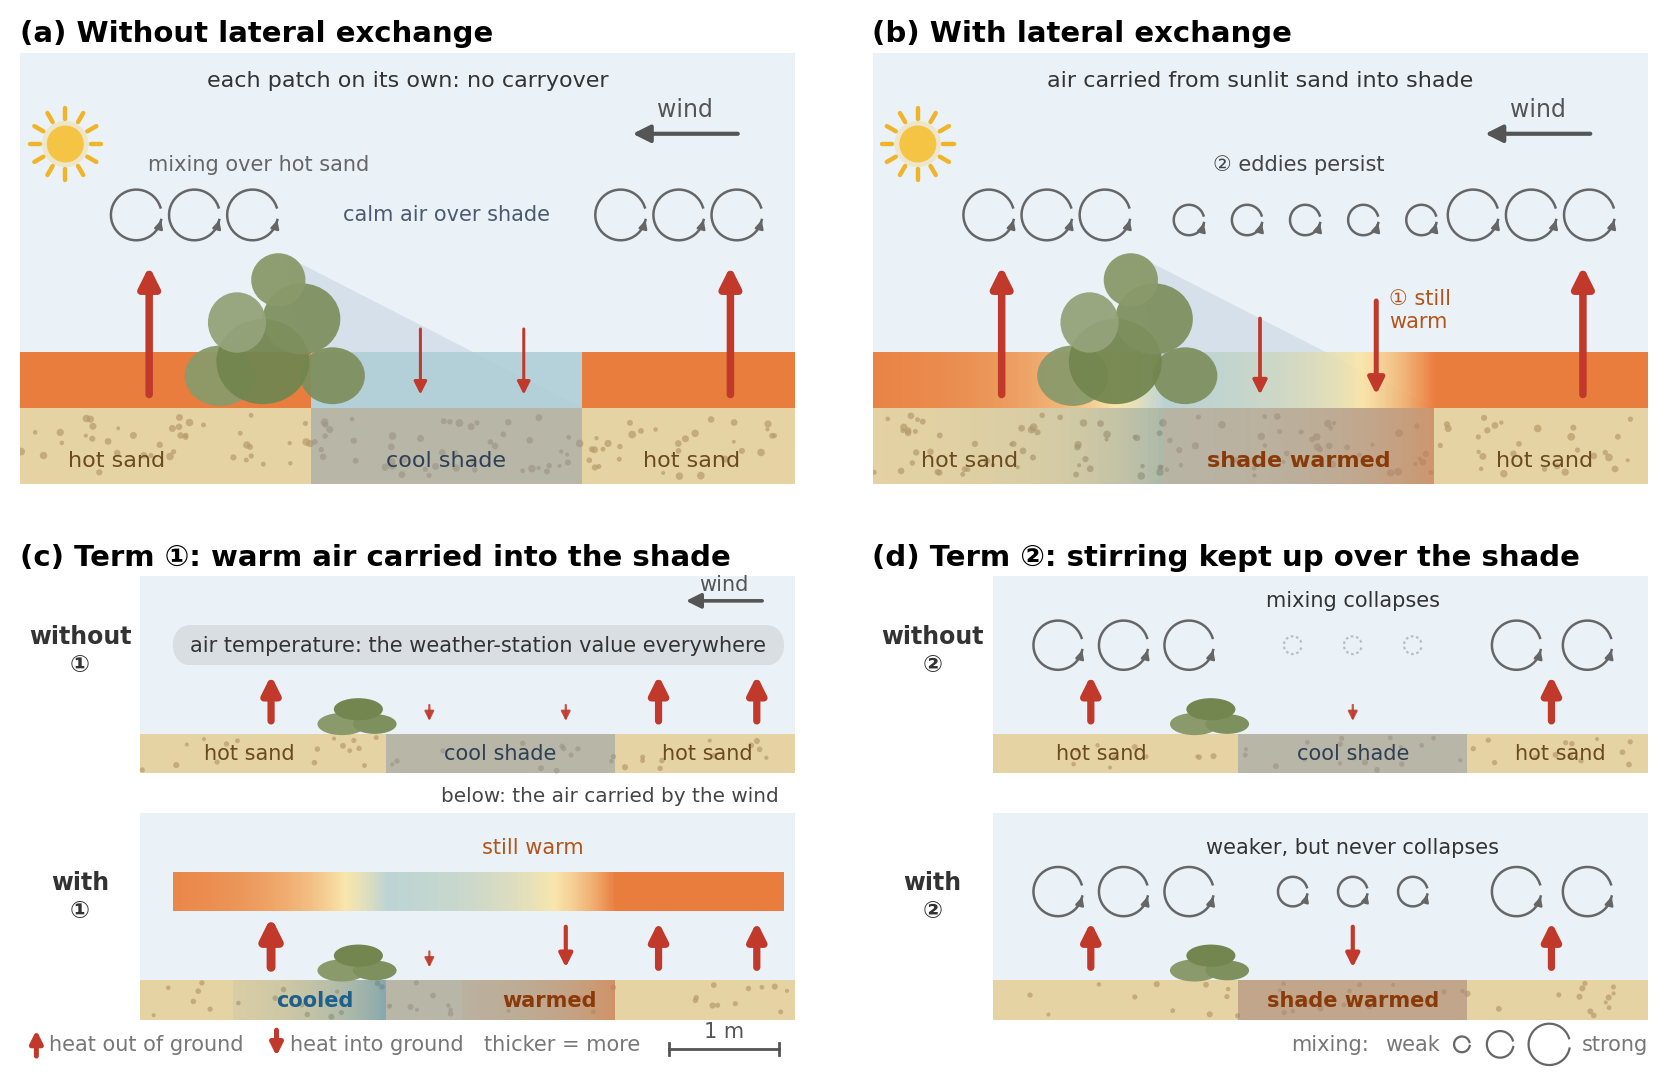
\includegraphics[width=0.85\textwidth]{schematic_lateral_vs_no_lateral.png}
    \caption{Schematic of lateral heat exchange across shadow margins in the physical energy-balance model. (a) In the uncoupled 1D model, each pixel exchanges heat independently with undisturbed reference air: hot sunlit sand generates convective turbulence, whereas stable conditions over cooler shaded ground reduce modeled turbulent exchange. (b) In the coupled 2D lateral model, wind carries air heated over upwind sunlit sand into adjacent shade (Term 1) while maintaining turbulent mixing generated over the surrounding terrain (Term 2), warming the shaded surface near its upwind edge. (c) Term 1 (advected air layer): wind advects a near-surface thermal anomaly with a relaxation distance of $\approx 0.7$~m at $2~\text{m s}^{-1}$ ($0.4$--$1.4$~m across flights). (d) Term 2 (turbulence floor): the heat-transfer coefficient over shade is bounded below by its neutral-stability value ($C_{H,\text{neutral}}$). Both processes act together in the sensible heat flux; open ground far from shade remains unchanged.}
    \label{fig:schematic_lateral}
\end{figure}

% \paragraph*{\textit{Independent Benchmark: microclimf}}
% To evaluate whether the limitations of 1D modeling are unique to our baseline formulation or represent a broader challenge across existing process-based software, we benchmarked our predictions against the independent package \textit{microclimf} \citep{maclean_2026}. \textit{microclimf} is an established mechanistic R package designed to simulate fine-scale landscape microclimates using a two-stage computational architecture:
% (1) a temporal point model (\texttt{runpointmodel}) that simulates the 1D surface energy balance hourly over the 24 hours preceding each drone flight, parameterizing soil heat flux from the running daily mean temperature; and
% (2) a spatial downscaling module (\texttt{runmicro}) that projects surface fluxes onto our 15~cm grid using high-resolution terrain geometry. The spatial module explicitly resolves 3D ray-traced direct solar beam shadowing across 24 radial azimuths on the DSM, diffuse skyview obstruction, and directional wind sheltering across eight compass bearings.
% 
% Crucially, while \textit{microclimf} accounts for sophisticated non-local terrain geometry (shadow casting and sky obstruction), its surface energy balance remains strictly uncoupled column-by-column: it calculates aerodynamic resistance and sensible heat flux independently at each pixel with ambient air, with zero horizontal transport of heated air or advected turbulence across patch boundaries. It therefore provides an ideal, independent mechanistic benchmark to evaluate whether non-local terrain geometry alone is sufficient to predict fine-scale thermal ecotones, or whether horizontal heat exchange is physically required.
% 
% Because \textit{microclimf} was developed and parameterized primarily for temperate, above-sea-level European landscapes, its default settings produced physical artifacts at our hyper-arid, below-sea-level site. To obtain a fair benchmark without modifying the package's core equations, we adapted five of its settings to the site; these adaptations are listed in Supplementary Section~S3.3.

\noindent Full mathematical derivations of the energy-balance equations, numerical solver discretizations, and parameter values are detailed in Supplementary Information Section~S3.

\subsection{Statistical Analysis}
\noindent We used generalized additive and generalized linear mixed-effects models (GAMMs and GLMMs) to test our two hypotheses across the held-out test submaps.

\paragraph*{\textit{Spatial Scaling and Diurnal Interaction GAMMs}}
To test Hypothesis~(1), we analyzed how anchored prediction error ($\text{MSE}$, in $^{\circ}\mathrm{C}^2$, seed-averaged per submap and microhabitat) varied with tile width across microhabitats and times of day. We fitted GAMMs using the \textit{bam} function in the \textit{mgcv} R package \citep{mgcv_2011, R_Core_Team} with a Gamma error distribution and log link function to account for strictly positive, right-skewed errors. The full model included separate penalized thin-plate regression smooths of tile width for each daypart ($s(\text{tile width}, \text{by} = \text{daypart}, k = 8)$), categorical fixed effects for microhabitat (open sand [reference] vs.\ canopy shade), daypart (morning: 06:00--07:00, midday: 08:00--16:00, evening: 17:00--18:00), and their interaction ($\text{microhabitat} \times \text{daypart}$), plus a random intercept for flight identity ($s(\text{flight}, \text{bs} = \text{"re"})$). We compared candidate smooth and interaction specifications using the Akaike Information Criterion (AIC; Supplementary Table~S2).

To estimate the tile width at which midday shade improvements leveled off, we fitted generalized nonlinear mixed-effects plateau models (Gamma distribution, log link) to the midday shaded-submap errors ($N = 27$ submaps across 6 midday test flights) using \textit{glmmTMB} \citep{brooks2017glmmtmb}. These models included tile width ($0.15$ to $12.15$~m) as the continuous predictor and random intercepts for flight and submap to account for repeated evaluations across tile widths. Using AIC, we compared quadratic- and linear-plateau models (each estimating a breakpoint tile width $X_0$ beyond which MSE no longer decreased) against non-plateau quadratic, linear, and intercept-only models. We also tested successive pairwise contrasts between adjacent tile widths using the \textit{emmeans} package \citep{Lenth2024emmeans} and evaluated simultaneous 95\% confidence bands of the GAMM first derivatives to identify where the slope of MSE with respect to tile width became indistinguishable from zero.

\paragraph*{\textit{Physical Feature and Network Ablation Modeling}}
To quantify the effect of permuting each map layer or ablating each network component during the midday flights (08:00--16:00), we fitted pairwise GAMMs (Gamma distribution, log link) in \textit{mgcv} comparing each ablated condition against the intact baseline model. Each GAMM included condition-specific smooths of tile width ($s(\text{tile width}, \text{by} = \text{condition})$), a fixed effect for condition, and a random intercept for flight identity. From these models, we estimated marginal MSE response ratios ($\text{MSE}_\text{ablated} / \text{MSE}_\text{intact}$) and 95\% confidence intervals using \textit{emmeans} \citep{Lenth2024emmeans}.

\paragraph*{\textit{Paired GLMM Evaluation of Physical Lateral Heat Exchange}}
To test Hypothesis~(2), we compared the 1D baseline model against the 2D coupled lateral model across all bare-ground pixels ($N = 3{,}109{,}545$) within the held-out $50\times50$~m test blocks of the 10 evaluation flights ($N = 36$ submaps with open-ground test pixels and $N = 32$ submaps with shaded-ground test pixels). To test whether the effect of lateral heat exchange differed between microhabitats while accounting for repeated measures across flights and submaps, we fitted a Gamma-log GLMM in \textit{glmmTMB} \citep{brooks2017glmmtmb}:
\begin{equation} \label{eq:glmm_lateral}
\log(\mu_{ijk}) = \beta_0 + \beta_1 \text{lateral}_i + \beta_2 \text{microhabitat}_j + \beta_3 (\text{lateral}_i \times \text{microhabitat}_j) + b_{\text{flight},k} + b_{\text{submap},jk},
\end{equation}
where $\mu_{ijk}$ is the expected submap MSE, $\text{lateral} \in \{\text{off}, \text{on}\}$ indicates the physical model configuration (1D baseline as reference), $\text{microhabitat} \in \{\text{open}, \text{shade}\}$ (open ground as reference), and $b_{\text{flight},k} \sim \mathcal{N}(0, \sigma^2_{\text{flight}})$ and $b_{\text{submap},jk} \sim \mathcal{N}(0, \sigma^2_{\text{submap}})$ are random intercepts for flight and submap. From the fitted GLMM, we computed habitat-specific marginal MSE ratios ($\text{MSE}_\text{with} / \text{MSE}_\text{without}$) and 95\% confidence intervals via \textit{emmeans} \citep{Lenth2024emmeans}. To verify that results did not depend on open-ground centering, we repeated the GLMM analysis on raw, uncentered predictions. All statistical scripts and model outputs are archived in the public repository (\url{https://github.com/levyofi/Sulami_et_al_2026}).

\section{RESULTS}


%\noindent Across all test submaps, the anchored mean squared error (MSE) decreased from 1.63 ± 0.95 (mean ± SD, $^{\circ}\mathrm{C}^2$) for the non-spatial $1\times1$ baseline to 1.43 ± 0.69 $^{\circ}\mathrm{C}^2$ at a tile size of 15 pixels, and remained between 1.42 and 1.51 $^{\circ}\mathrm{C}^2$ for all larger tiles. This overall average, however, conceals strong differences between dayparts and microhabitats, which we examine next. For comparison, the unanchored MSE was dominated by scene-level offsets on the held-out flights (squared bias of 3.6--6.6 $^{\circ}\mathrm{C}^2$ versus an anchored error of about 1.5 $^{\circ}\mathrm{C}^2$; Section~S2.3), and these offsets, not spatial context, produced the apparent dependence of unanchored error on tile size.

\subsection{The Importance of Spatial Information Across Microhabitats and Dayparts}

\noindent Surrounding terrain context significantly reduced ground temperature prediction errors at midday, but not in the morning or evening (Fig.~\ref{fig:tile_size_vs_microhabitat_daypart}). Among candidate GAMMs, the model with daypart-specific tile-width smooths and a $\text{microhabitat} \times \text{daypart}$ interaction (Model M4) had the lowest AIC ($\Delta\text{AIC} \ge 14.9$ relative to simpler models and $\Delta\text{AIC} > 400$ relative to daypart-invariant smooths; Supplementary Table~S2). Expanding tile width reduced anchored MSE at midday (\textit{Midday smooth}: $\text{edf} = 4.02$, $F = 9.61$, $p < 0.001$), whereas the morning and evening smooths were linear and non-significant (\textit{Morning}: $\text{edf} = 1.00$, $F = 1.20$, $p = 0.27$; \textit{Evening}: $\text{edf} = 1.00$, $F = 1.76$, $p = 0.19$).

At midday, increasing tile width from a single pixel ($0.15$~m) to 15 pixels ($2.25$~m) reduced marginal MSE in canopy shade by 38.4\%, from $4.64^{\circ}\mathrm{C}^2$ (95\% CI: $3.88$--$5.40$) to $3.07^{\circ}\mathrm{C}^2$ ($2.63$--$3.51$), and to $2.86^{\circ}\mathrm{C}^2$ ($2.40$--$3.31$) at 31 pixels ($4.65$~m), with no further reduction at larger widths. In open sand, midday MSE similarly dropped by 38.5\%, from $2.41^{\circ}\mathrm{C}^2$ ($2.02$--$2.79$) at 1 pixel to $1.59^{\circ}\mathrm{C}^2$ ($1.37$--$1.82$) at 15 pixels and $1.48^{\circ}\mathrm{C}^2$ ($1.25$--$1.71$) at 31 pixels. By contrast, morning and evening MSEs were already low at the single-pixel baseline (morning open: $1.00^{\circ}\mathrm{C}^2$, shade: $2.68^{\circ}\mathrm{C}^2$; evening open: $0.70^{\circ}\mathrm{C}^2$, shade: $2.02^{\circ}\mathrm{C}^2$) and did not change significantly with tile width. These low morning and evening errors match the small temperature variance observed across the ground surface at low sun angles ($0.7$--$1.0^{\circ}\mathrm{C}^2$ vs.\ $4.0^{\circ}\mathrm{C}^2$ at midday), when little temperature contrast exists relative to open sand. Across all tile widths, parametric GAMM terms showed that MSE was higher in canopy shade than in open sand (\textit{shade main effect}, log scale: $0.98 \pm 0.08$, $t = 11.81$, $p < 0.001$), and that the relative log-ratio between shade and open MSE was smaller at midday than in the morning (\textit{shade} $\times$ \textit{midday}: $-0.33 \pm 0.10$, $t = -3.36$, $p < 0.001$; \textit{shade} $\times$ \textit{evening}: $0.08 \pm 0.12$, $t = 0.69$, $p = 0.49$).

To estimate the tile width at which midday shade improvements leveled off, we compared nonlinear plateau models across the midday shaded submaps. A quadratic-plateau model outperformed linear-plateau ($\Delta\text{AIC} = 4.0$), quadratic polynomial ($\Delta\text{AIC} = 50.1$), linear ($\Delta\text{AIC} = 105.6$), and intercept-only ($\Delta\text{AIC} = 150.6$) models. The fitted breakpoint occurred at a tile width of $X_0 = 14.5$ pixels ($2.18$~m at $0.15$~m/pixel, just below the tested $15\times15$ tile of $2.25$~m, or $\approx 1.1$~m outward from the target pixel; 95\% profile-likelihood CI: $11.5$--$18.5$ pixels, corresponding to $1.73$--$2.78$~m at $0.15$~m/pixel [$1.78$--$2.87$~m at $0.155$~m/pixel], $p < 0.001$), reaching an estimated plateau MSE of $2.33^{\circ}\mathrm{C}^2$. Successive contrasts between adjacent tested tile sizes supported this breakpoint: MSE decreased significantly from $9\times9$ to $15\times15$ pixels ($z = -2.83$, adjusted $p < 0.05$) but showed no significant change from $15\times15$ to $21\times21$ pixels ($z = 0.74$, adjusted $p = 1.00$), and simultaneous 95\% confidence bands of the GAMM first derivative included zero from $31\times31$ pixels ($4.65$~m tile width, $\approx 2.3$~m from the target pixel) onward.

\begin{figure}[!h]
    \centering
    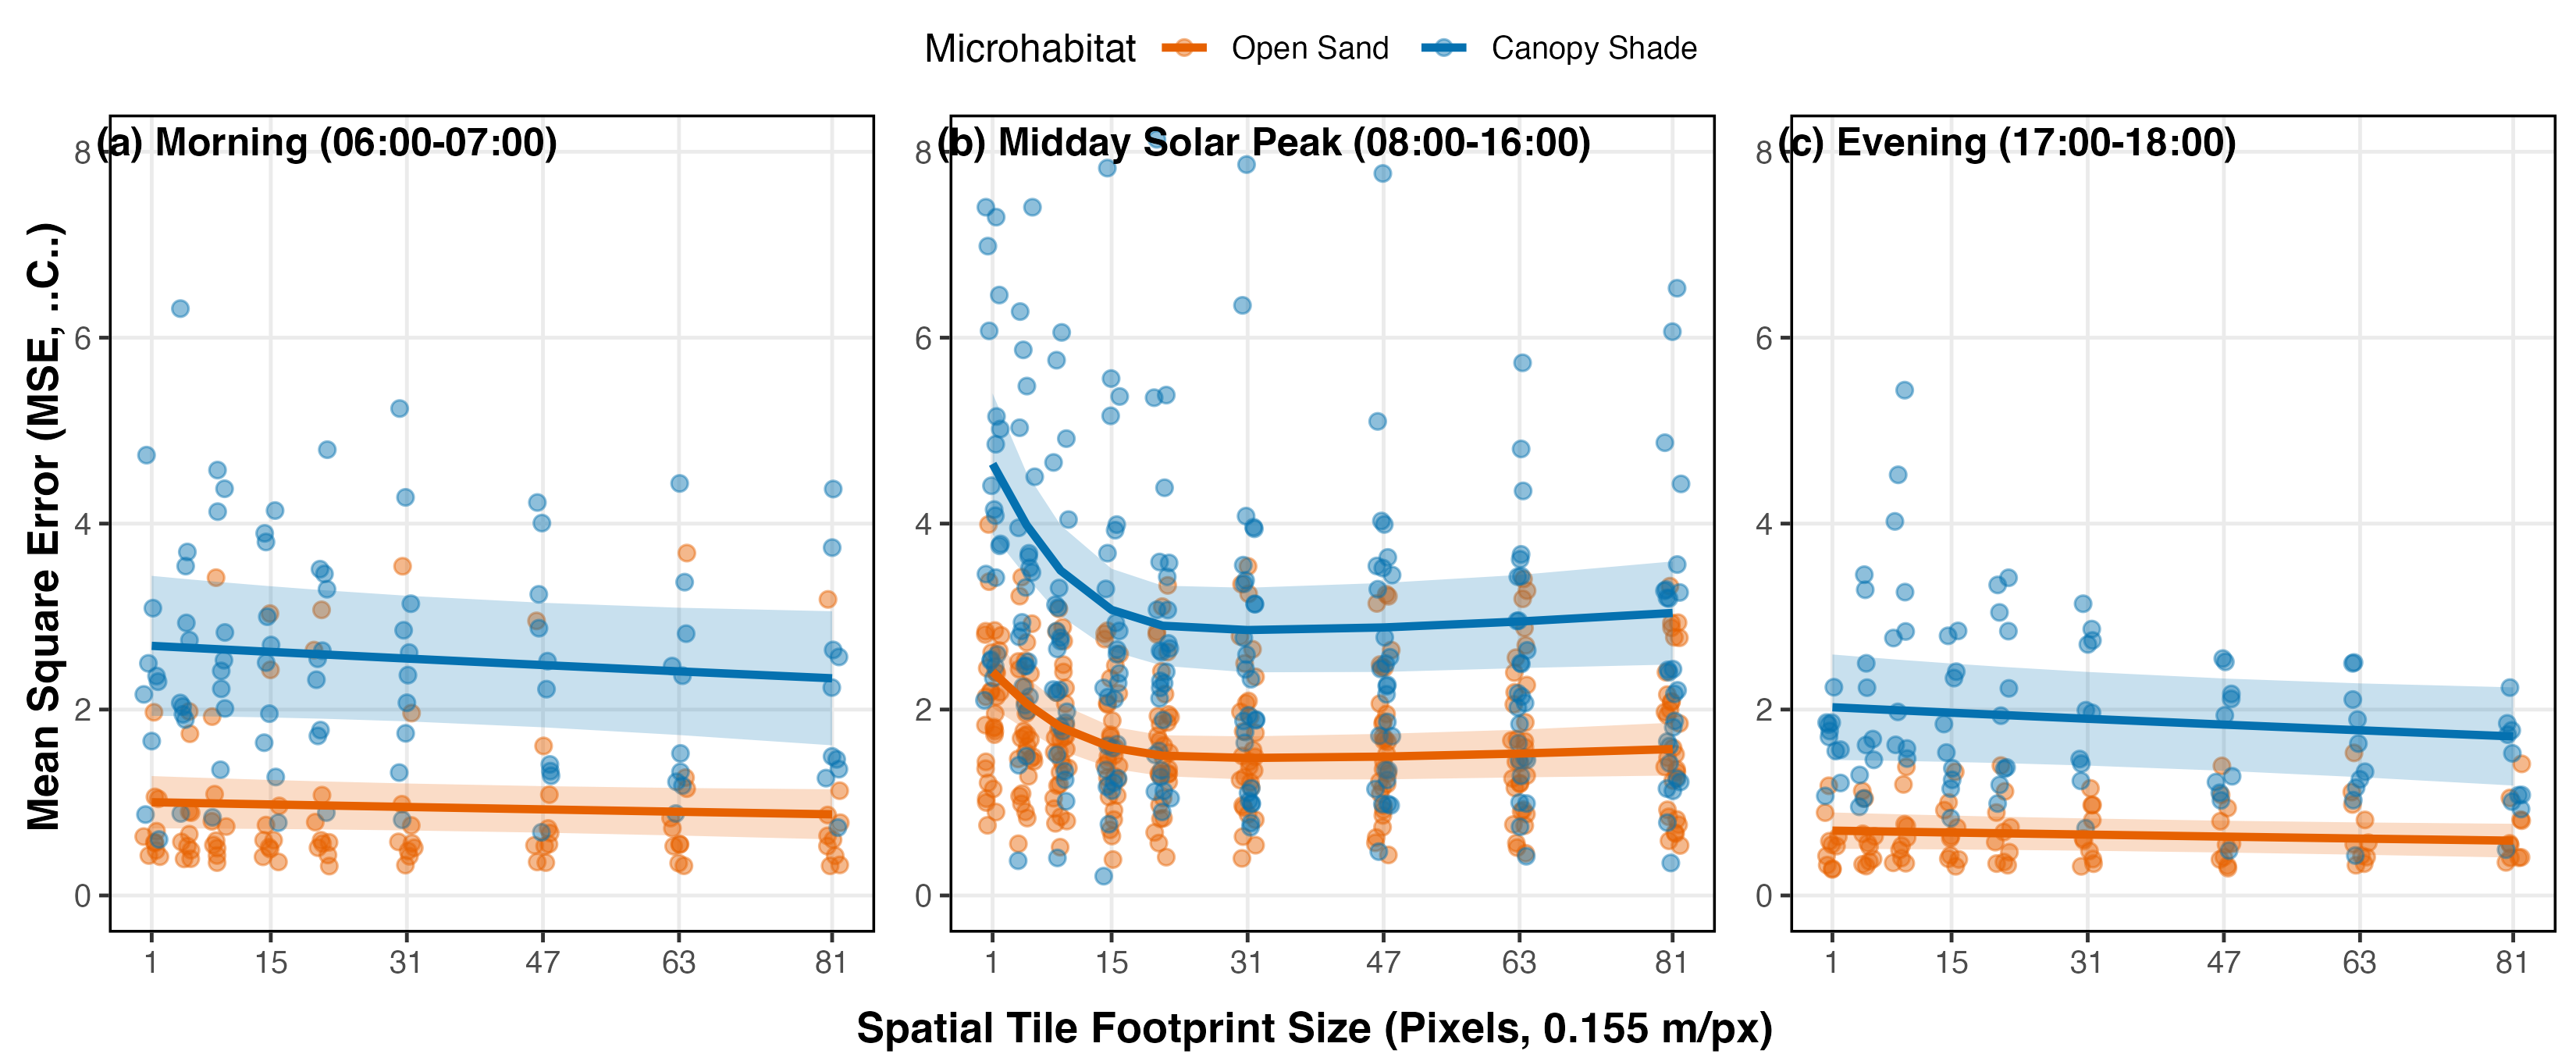
\includegraphics[width=1\textwidth]{Figure_4_diurnal_gamm_scaling_self_anchored.png}
    \caption{Surrounding terrain reduces ground temperature prediction error at midday but not in the morning or evening. Panels show anchored mean squared error (MSE, in $^{\circ}\mathrm{C}^2$, relative to mean open ground; Eq.~\ref{eq:anchored_error}) across test submaps (points, seed-averaged) and GAMM marginal response curves (lines with 95\% confidence bands) as a function of square tile width (pixels, $0.15$~m/pixel) in open sand (orange) and canopy shade (blue) during: (a) morning (06:00--07:00), (b) midday (08:00--16:00), and (c) evening (17:00--18:00). Midday error decreases up to tile widths of 15--21 pixels ($2.25$--$3.15$~m) and stabilizes by 31 pixels ($4.65$~m), whereas morning and evening surfaces are nearly isothermal relative to open ground.}
    \label{fig:tile_size_vs_microhabitat_daypart}
\end{figure}

\subsection{Physical Feature and Network Ablation at Midday}

\noindent Because surrounding terrain improved predictions at midday (Section~3.1), we evaluated the feature permutations and network ablations across the midday test flights (08:00--16:00; Fig.~\ref{fig:feature_ablation}; Supplementary Table~S3). Pairwise GAMMs showed that permuting any of the five spatial map layers significantly increased midday anchored MSE, with radiation and terrain geometry having the largest effects.

Incoming solar radiation was the input whose permutation caused the largest error increase across all tile widths, raising midday anchored MSE by 84.0\% (MSE ratio $= 1.840 \pm 0.082$, $t = 13.60$, $p < 0.001$, from $1.64$--$2.14^{\circ}\mathrm{C}^2$ to $2.98$--$4.00^{\circ}\mathrm{C}^2$; Fig.~\ref{fig:feature_ablation}a). Skyview factor was the second most influential layer: permuting skyview values increased midday MSE by 28.8\% (MSE ratio $= 1.288 \pm 0.053$, $t = 6.15$, $p < 0.001$; Fig.~\ref{fig:feature_ablation}b). Permuting the binary shade layer and obstacle height ($\text{DSM} - \text{DTM}$) also significantly degraded midday predictions, increasing anchored MSE by 21.2\% (MSE ratio $= 1.212 \pm 0.055$, $t = 4.25$, $p < 0.001$; Fig.~\ref{fig:feature_ablation}d) and 13.3\% (MSE ratio $= 1.133 \pm 0.039$, $t = 3.59$, $p < 0.001$, reaching $+28.9\%$ at $5\times5$ pixels; Fig.~\ref{fig:feature_ablation}c), respectively.

Permuting the vegetation index (TGI) caused the smallest but still statistically significant error increase among the five map layers ($+9.3\%$, MSE ratio $= 1.093 \pm 0.040$, $t = 2.40$, $p = 0.017$; Fig.~\ref{fig:feature_ablation}e). Because vegetated pixels ($\text{TGI} > 0.04$) were excluded from the evaluation targets, this result indicates that TGI in surrounding pixels improved bare-ground predictions near shrubs; surrounding TGI may help the network distinguish live shrubs from rocks of similar height, reflecting differences in canopy shading structure or vegetation-associated cooling.

Among the network components, utilizing surrounding terrain depended strongly on the spatial pooling step, which summarizes the 32 feature maps across the tile using their mean and maximum. At the single-pixel baseline ($1\times1$), disabling pooling had no effect because the center pixel, tile mean, and tile maximum are identical ($2.05^{\circ}\mathrm{C}^2$ MSE in both configurations). For multi-pixel tiles, however, the intact network used pooled tile summaries to lower midday MSE to $1.64$--$1.73^{\circ}\mathrm{C}^2$, whereas disabling spatial pooling increased MSE by 59.9\% overall (MSE ratio $= 1.599 \pm 0.090$, $t = 8.33$, $p < 0.001$, reaching $3.18^{\circ}\mathrm{C}^2$ at the largest tiles; Supplementary Fig.~S1a). By contrast, disabling the FiLM weather-scaling layers ($-4.4\%$, $p = 0.16$) or setting all eight weather inputs to zero ($-3.3\%$, $p = 0.30$) had no significant effect on anchored MSE (Supplementary Fig.~S1b,c; Supplementary Table~S3). Because weather-station readings are constant across a flight, they primarily shift the scene-wide baseline temperature (which is removed by open-ground centering) rather than within-scene temperature contrasts.

\begin{figure}[!h]
    \centering
    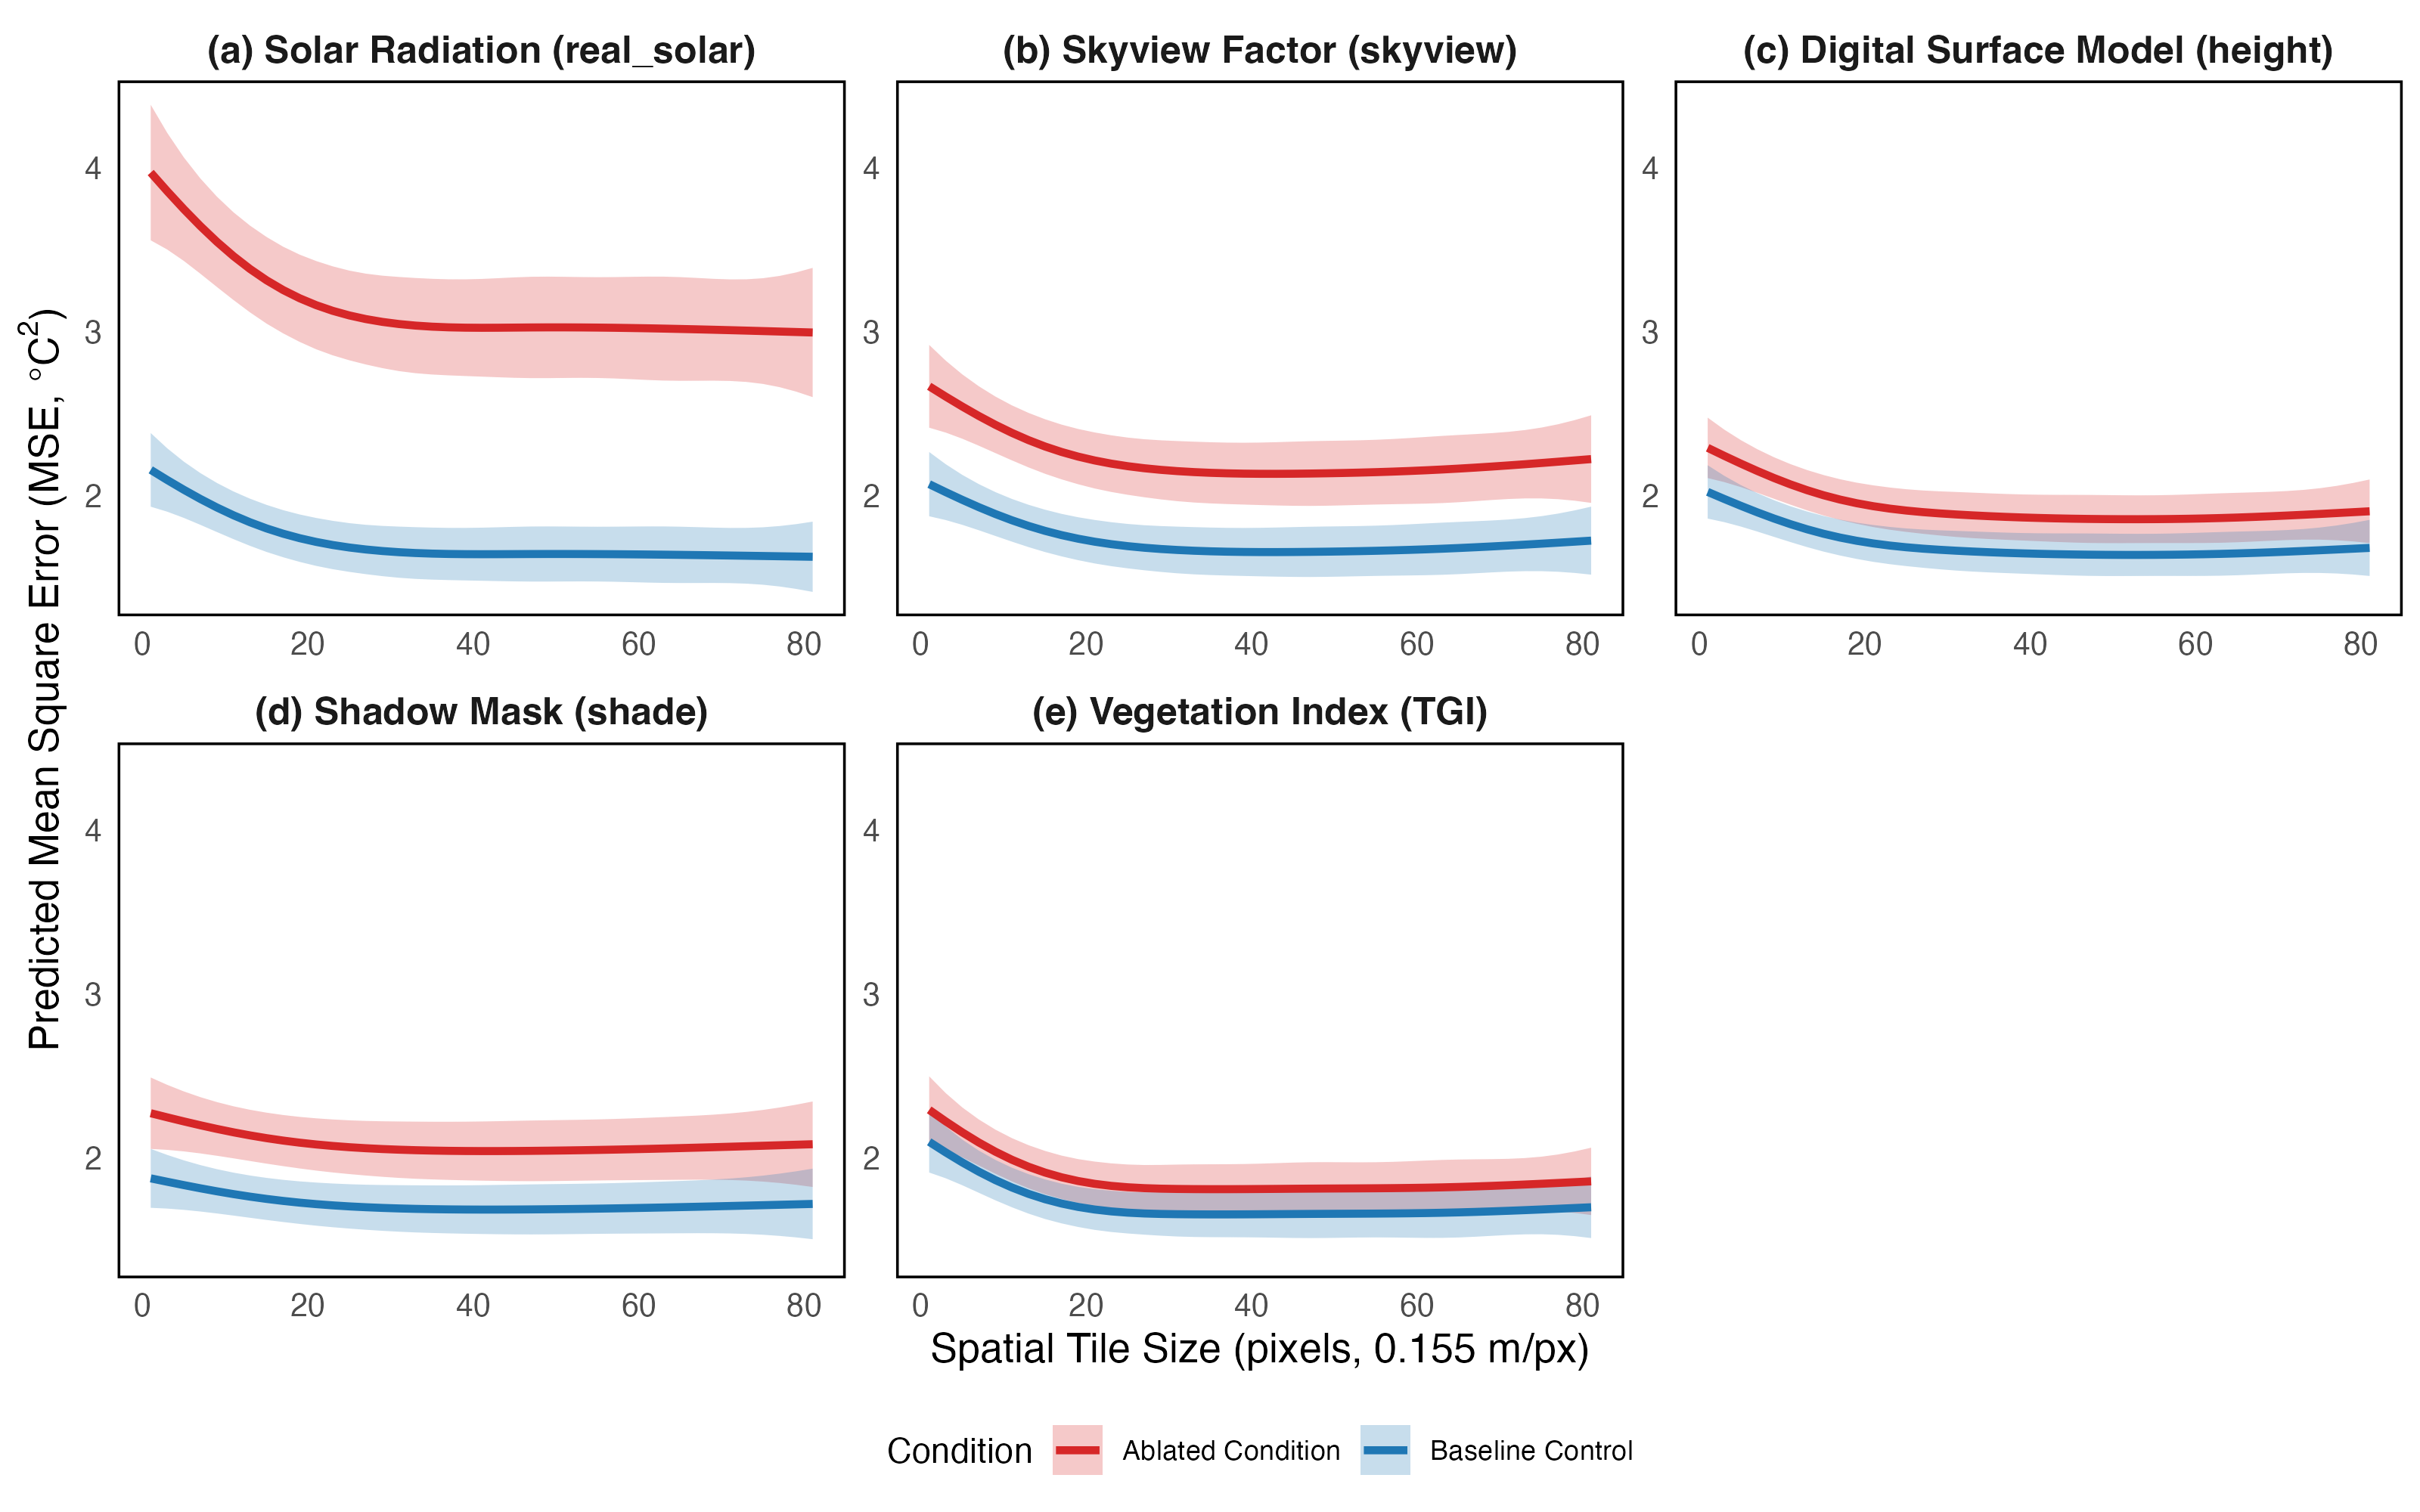
\includegraphics[width=1\textwidth]{Figure 6.png}
    \caption{Pairwise physical feature permutations at midday (08:00--16:00). Panels show fitted GAMM marginal curves and 95\% confidence bands for anchored MSE (in $^{\circ}\mathrm{C}^2$, relative to mean open ground; Eq.~\ref{eq:anchored_error}) comparing the intact baseline model (blue) against models with one permuted map layer (red) across tile widths up to 81 pixels ($12.15$~m; $0.15$~m/pixel): (a) incoming solar radiation ($+84.0\%$ MSE increase, $p < 0.001$), (b) skyview factor ($+28.8\%$ MSE increase, $p < 0.001$), (c) obstacle height ($\text{DSM} - \text{DTM}$; $+13.3\%$ MSE increase, $p < 0.001$), (d) binary shade ($+21.2\%$ MSE increase, $p < 0.001$), and (e) vegetation index (TGI; $+9.3\%$ MSE increase, $p = 0.017$).}
    \label{fig:feature_ablation}
\end{figure}

\subsection{Coupled Lateral Heat Exchange Reduces the Shade-Cooling Bias}

\noindent Adding horizontal heat advection and a neutral-stability turbulent mixing floor to the physical energy-balance model substantially reduced prediction errors in shaded ground, while changing open-ground predictions only slightly (Fig.~\ref{fig:lateral_on_off_boxplot}; Supplementary Table~S5).

In shaded ground, the coupled 2D lateral model lowered MSE in 31 of the 32 shaded test submaps (96.9\%; Fig.~\ref{fig:lateral_on_off_boxplot}b). Across shaded submaps, median MSE decreased by 70.8\% (median MSE ratio $= 0.292$), and mean MSE fell from $8.81^{\circ}\mathrm{C}^2$ under the 1D baseline model to $2.68^{\circ}\mathrm{C}^2$ with lateral heat exchange (Supplementary Table~S5).

The reduction in error was significantly larger in shade than in open ground ($\text{lateral} \times \text{microhabitat}$ interaction: $\beta_3 = -0.987 \pm 0.198$, $z = -4.97$, $p < 0.001$). Based on GLMM marginal estimates, lateral heat exchange reduced shaded-ground MSE by 70.2\% (MSE ratio $= 0.298$, 95\% CI: $0.225$--$0.396$, $z = -8.34$, $p < 0.001$). Over uniform open sand far from shadows, the advected air anomaly approaches zero ($T_{\text{air}} \to T_{\text{air,uniform}}$; Supplementary Section~S3.2), so open-ground MSE changed much less and the marginal reduction was not statistically significant (MSE ratio $= 0.801$, 95\% CI: $0.614$--$1.044$, $z = -1.64$, $p = 0.10$; mean MSE $= 1.05^{\circ}\mathrm{C}^2$ without lateral exchange vs.\ $0.89^{\circ}\mathrm{C}^2$ with lateral exchange; Fig.~\ref{fig:lateral_on_off_boxplot}a).

Repeating the GLMM analysis on raw, uncentered predictions showed that the shaded-ground improvement did not depend on removing the open-ground offset. Without offset removal, lateral heat exchange reduced shaded-ground MSE by 54.9\% (MSE ratio $= 0.451$, 95\% CI: $0.297$--$0.683$, $p < 0.001$), while open-ground MSE remained unchanged (MSE ratio $= 1.006$, 95\% CI: $0.688$--$1.470$, $p = 0.98$; Supplementary Table~S5).

\begin{figure}[!h]
    \centering
    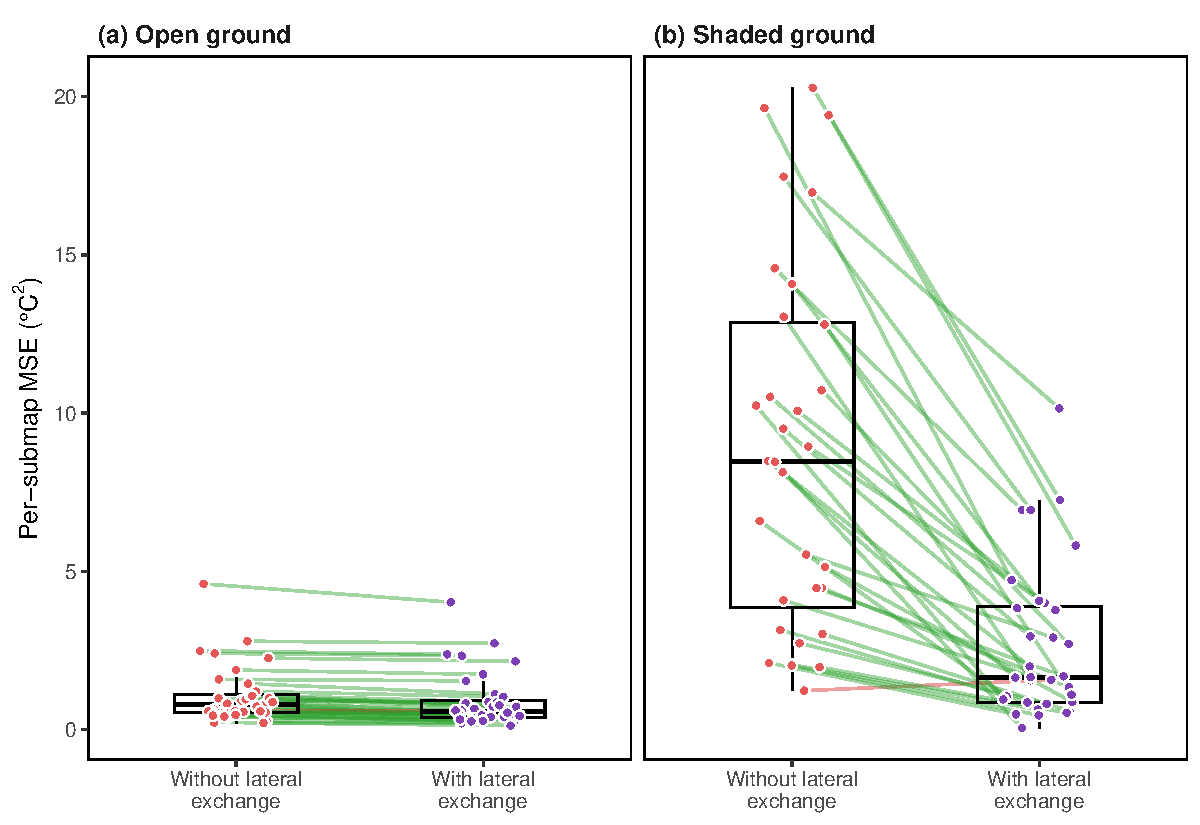
\includegraphics[width=0.88\textwidth]{Figure_lateral_on_off_paired_boxplot.pdf}
    \caption{Paired submap prediction error (anchored MSE in $^\circ\mathrm{C}^2$, relative to mean open ground; Eq.~\ref{eq:anchored_error}) of the physical energy-balance model without versus with coupled lateral heat exchange across held-out test blocks ($N = 36$ open and $N = 32$ shaded submaps across 10 evaluation flights): (a) Open ground and (b) Shaded ground. Points represent individual submaps; lines connect paired evaluations of the same submap (green where lateral exchange lowered MSE, red where it raised MSE). Boxplots show the median, interquartile range (IQR), and $1.5\times\text{IQR}$ whiskers. Including horizontal heat advection and a neutral-stability turbulent mixing floor reduced MSE in 31 of 32 shaded submaps (median MSE ratio $= 0.292$; $-70.2\%$ GLMM marginal MSE reduction, $p < 0.001$), while open-ground MSE changed only modestly (median MSE ratio $= 0.804$, GLMM $p = 0.10$).}
    \label{fig:lateral_on_off_boxplot}
\end{figure}

\section{DISCUSSION}
\subsection{Deep Learning as a Diagnostic of Spatial Microclimate Context}

\noindent
Most physically based microclimate models compute surface temperatures independently for each grid cell, relying on 1D vertical energy balances that omit horizontal heat exchange in the near-surface air \citep{briscoe_2023, maclean_2026}. By varying the input tile width of a CNN while holding its parameter count constant, we quantified the spatial scale over which surrounding terrain improves midday ground temperature predictions. Midday MSE decreased by about 38\% as tile width expanded from a single pixel to a fitted plateau width of 1.7--2.8~m (extending 0.9--1.4~m outward from the target pixel), with no further improvement beyond 4.7~m (2.3~m from the target pixel). These dimensions match the canopy widths of perennial shrubs (1--3~m) and their cast shadows (0.5--2.5~m) at our desert site. Omitting interactions across these scales produced substantial prediction errors: single-pixel CNN inputs missed roughly 38\% of the reducible midday MSE, and our 1D physical baseline model predicted shaded bare ground 5--12$^\circ$C cooler than sunlit sand, compared with an observed difference of 1--3$^\circ$C.

In machine learning applications, input tile size is typically treated as a hyperparameter tuned to minimize validation error, after which other sizes are discarded. Here, keeping the network architecture and parameter count (~55,700 parameters) identical across tile widths from $0.15$ to $12.15$~m allowed us to use tile width as an empirical probe of spatial scale. Because predictions were evaluated on spatial blocks and flights excluded from training, the error reduction with increasing tile width reflects information carried by surrounding terrain features rather than increased model capacity or site memorization. The leveling off of accuracy gains beyond 1.7--2.8~m tile width indicates that the spatial independence assumed by 1D microclimate models breaks down primarily across the 1--3~m margins of individual shrubs and boulders.

\subsection{Spatial Context Varies Across Times of Day and Environmental Layers}

\noindent Larger input tiles improved CNN predictions at midday, when sunlit sand and shaded ground differed most in temperature, whereas morning and evening predictions showed no significant benefit from surrounding terrain (Fig.~\ref{fig:tile_size_vs_microhabitat_daypart}). This diurnal pattern reflects the surface energy balance of the desert ground. Under intense midday solar heating, steep temperature gradients between exposed sand and adjacent shade drive lateral advection of warm air and turbulent mixing across shadow boundaries. In the morning and evening, by contrast, low solar angles leave the ground surface nearly isothermal relative to open sand (spatial variance $<1.0^{\circ}\mathrm{C}^2$), so surrounding terrain adds little information beyond local pixel properties.

Beyond time of day, feature permutations showed that midday predictions relied most on incoming solar radiation, skyview factor, and shadow boundaries, and least on vegetation greenness (Fig.~\ref{fig:feature_ablation}). This ranking of map layers matches the desert surface energy balance, where shortwave heating of exposed sand and unobstructed longwave cooling govern surface temperatures and establish sharp contrasts across shadow edges. Capturing these cross-boundary contrasts in the CNN required spatial pooling (tile-wide mean and maximum) to summarize surrounding terrain, as disabling pooling increased midday MSE by 59.9\% (Supplementary Fig.~S1a). By contrast, ablating the flight-level weather inputs or FiLM layers had little effect on anchored MSE, because uniform station readings shift the whole-scene baseline temperature rather than local contrasts within a scene.

\subsection{Implications for Physically Based Microclimate Models}

\noindent
Our results highlight a key limitation of assuming horizontal independence in fine-scale microclimate models. Process-based frameworks such as \textit{NicheMapR} \citep{kearney_2017}, \textit{microclima} \citep{maclean_2019}, and \textit{microclimf} \citep{maclean_2026} calculate radiative shading from surrounding terrain but solve turbulent heat exchange column by column, assuming infinite uniform fetch \citep{brutsaert_1982}. In our 1D baseline model \citep{Itzkovitch2025}, this assumption caused a systematic overestimation of midday shade cooling: the 1D model predicted shaded ground 5--12$^\circ$C cooler than sunlit sand, whereas drone thermal maps showed an observed difference of 1--3$^\circ$C. Because an isolated 1D column cuts off shaded ground from warm air advected off upwind sunlit sand and suppresses turbulent mixing under stable local stratification, it underestimates sensible heat transfer into small shade patches.

Adding horizontal heat advection and a neutral-stability turbulent exchange floor to our physical model reduced shaded-ground MSE by 70.2\% across the evaluation flights (lowering error in 31 of 32 shaded submaps), primarily by warming shaded ground within the first 0.4--1.4~m of the upwind shadow edge (Fig.~\ref{fig:lateral_on_off_boxplot}). This advective relaxation distance (0.4--1.4~m) aligns qualitatively with the CNN's plateau half-width (0.9--1.4~m outward from the target pixel, corresponding to a 1.7--2.8~m tile width). Although these two quantities represent different model properties (one an empirical input window aggregating radiative and topographic context, the other a calibrated directional relaxation length), both indicate that surrounding sunlit terrain warms small desert shade patches over scales of 1--3~m.

Beyond 2D gridded simulations, these findings suggest a practical, though currently untested, approximation for point-based 1D microclimate models such as \textit{NicheMapR} \citep{kearney_2017}, which typically run unshaded and shaded columns to bound available thermal environments. When shaded refuges consist of small isolated patches (1--3~m shrubs or boulders) rather than continuous canopy, a 1D shaded column overestimates cooling because it assumes infinite shaded fetch. Much of the lateral warming could potentially be approximated without a 2D grid by first running the unshaded column, and then running the shaded column using a wind- and patch-width-weighted blend of the unshaded near-surface air temperature while maintaining neutral turbulent mixing.

\subsection{Combining Empirical Diagnostics and Physical Microclimate Models}

\noindent
More broadly, our workflow shows how fixed-capacity CNNs can help diagnose spatial processes that physical models omit. Varying input tile width while holding the network architecture and parameter count constant identified the spatial scale at which surrounding terrain improved predictions, guiding the formulation of our 2D lateral heat-exchange model. Looking ahead, a natural next step is to combine a physical energy-balance model directly with a learned spatial correction based on surrounding terrain \citep{wesselkamp_2024, levy_2024, Alujevic2025, deck_2026}. Such a hybrid model could retain conservation laws and out-of-sample robustness from the physical equations while learning sub-grid spatial effects that are difficult to parameterize, similar to modular land-surface frameworks such as \textit{ClimaLand} \citep{deck_2026, maclean_2026}. Any learned spatial correction should be tested across independent sites and weather regimes to verify that it generalizes beyond its training domain.

\subsection{Limitations and Future Directions}

\noindent
Improved CNN predictions with larger tiles show that surrounding terrain features contain useful predictive information, but they do not by themselves isolate a single physical heat-transfer mechanism. Because surrounding tiles contain correlated geometric and radiative signals, we paired the CNN analysis with feature permutations and a 2D energy-balance model, which together support key roles for radiation and lateral heat exchange across shadow boundaries. Directly testing the modeled horizontal heat fluxes in the field will require fine-scale measurements of air temperature, wind speed, and turbulent heat flux across shrub shade boundaries.

While the CNN was evaluated strictly out of sample on held-out spatial blocks and flights, some coefficients in process-based microclimate models cannot be measured directly and require empirical calibration \citep{briscoe_2023}. In our 2D physical model, the roughness length ($z_0 = 0.03$~m) was taken from published values for sparse scrub \citep{oke_1987}, and three lateral transport parameters ($L_g$, $L_e$, and $\phi$) were calibrated against shade-edge transects from two of the ten evaluation flights (23 September 2019 at 14:10 and 15:10; Supplementary Table~S4). The shaded-ground gains on those two flights are therefore not fully out of sample, although the lateral model also reduced shaded-ground MSE across the remaining eight uncalibrated test flights (lowering error in 31 of 32 shaded submaps overall).

Because the CNN was trained and evaluated on temperatures centered on each submap's open-ground mean, predicting absolute temperatures at a new site or under unseen weather conditions requires an open-ground reference temperature. On held-out test flights with wind directions outside the training range, uncentered CNN predictions exhibited scene-wide biases (squared biases of 3.6--6.6$^\circ\text{C}^2$; Supplementary Section~S2.3). In practical applications, this open-ground baseline can be supplied either by an on-site sensor over exposed ground or by coupling the CNN's local spatial anomalies to a 1D physical energy-balance model.

In addition, our CNN analysis used square tiles centered on the target pixel, whereas horizontal heat advection is directional and follows the prevailing wind. Extending the network to align input tiles or convolutional filters with the wind vector could separate upwind fetch effects from downwind wakes. Our thermal measurements also share the constraints of drone-based infrared thermography: uncooled thermal cameras have a nominal absolute uncertainty of $\pm 5^\circ$C (requiring station calibration) and cannot see through foliage, so shaded test pixels in our dataset represent bare ground ($\text{TGI} < 0.04$) cast in shadow beside shrubs and rocks rather than soil directly beneath dense canopies. Within each flight, however, the sensor's relative thermal sensitivity ($<0.1^\circ$C) resolves local temperature contrasts, and the consistency of the spatial scaling curves across 10 test flights from multiple campaigns supports a landscape signal rather than within-flight drift. Finally, our study covered a single hyper-arid desert site with sparse shrubs. The 1.7--2.8~m plateau width estimated here reflects the dimensions of desert shrubs and shadows; in forests or wetter ecosystems with taller canopies and stronger evapotranspiration \citep{gril_2023}, spatial coupling is likely to act over larger distances that remain to be quantified.

\section{CONCLUSIONS}
\noindent
Varying the input tile width of a fixed-capacity CNN showed that surrounding terrain improves midday ground temperature predictions at our desert site up to a plateau width of 1.7--2.8~m (0.9--1.4~m from the target pixel), with no further improvement beyond 4.7~m. Within this surrounding neighborhood, permutation tests indicated that the network relied primarily on incoming solar radiation, skyview factor, and shade boundaries. Representing the resulting cross-boundary heat transport in a physical energy-balance model through near-surface horizontal advection and neutral turbulent mixing reduced shaded-ground MSE by 70.2\%. Together, these empirical and physical results show that the column-by-column independence assumption breaks down across small shade patches and illustrate how fixed-capacity neural networks can help identify missing spatial processes in microclimate models.


\subsection*{Data, Materials, and/or Code Availability}
\noindent Should the manuscript be accepted, the data and code with full equations will be archived in an appropriate public repository (e.g., Dryad, Figshare, or Zenodo) and the data DOI will be included at the end of the article. For review purposes, the code and sample data can be found in \url{https://github.com/levyofi/Sulami_et_al_2026}.

\subsection*{Authors' Contributions}
\noindent All authors conceived and designed the study, wrote the first draft and participated in revising the manuscript. OL collected the data and contributed mentorship. IS and AI contributed modeling and validation.

\section*{Acknowledgments}
\noindent We thank Simon Jamison for logistical assistance.

\newpage

\bibliography{references}

\end{document}